\documentclass[12pt,a4paper]{article}
\usepackage[utf8]{inputenc}
\usepackage[spanish]{babel}
\usepackage{amsmath,amsfonts,amssymb}
\usepackage{graphicx}
\usepackage{booktabs}
\usepackage{longtable}
\usepackage{array}
\usepackage{geometry}
\usepackage{fancyhdr}
\usepackage{natbib}
\usepackage{hyperref}
\usepackage{setspace}
\usepackage{threeparttable}
\usepackage{dcolumn}
\usepackage{multirow}
\usepackage{pdflscape}
\usepackage{afterpage}
\usepackage{capt-of}
\usepackage{float}
\usepackage{subcaption}

\geometry{margin=2.5cm}
\onehalfspacing

\title{\textbf{Replicación y Extensión de Pavia et al. (2017): \\Evaluación de la Calidad de las Añadas de la Contabilidad Nacional Trimestral Española con Análisis del COVID-19}}

\author{
    Manuel A. Hidalgo-Pérez\thanks{Universidad Pablo de Olavide, Sevilla. Email: mhidper@upo.es} \\ 
    \textit{Universidad Pablo de Olavide} \\[0.5em]
    \and
    Leandro Navarro Pablo\thanks{Autoridad Independiente de Responsabilidad Fiscal (AIReF). Email: lnavarro@airef.es} \\
    \textit{AIReF}
}

\date{\today}

\begin{document}

\maketitle

\begin{abstract}
\noindent Este trabajo presenta una replicación completa y una extensión del análisis de Pavia et al. (2017) sobre la calidad de las añadas de la Contabilidad Nacional Trimestral (CNTR) española. Replicamos exactamente su metodología para el período 2005-2016 y extendemos el análisis hasta 2025, incluyendo el período de la pandemia del COVID-19. Nuestra replicación valida los hallazgos originales de que las estimaciones del cuarto trimestre exhiben menores errores de revisión para las tasas de crecimiento interanuales. La extensión revela que el COVID-19 generó factores de amplificación de 2,94x comparado con períodos normales, mientras que la crisis de deuda soberana mostró la mayor amplificación (3,59x). Implementamos el análisis en código Python de acceso abierto, asegurando la reproducibilidad completa y proporcionando una base para futuras investigaciones sobre evaluación de calidad de cuentas nacionales.

\noindent \textbf{Palabras clave:} Contabilidad Nacional, Revisiones de Datos, Replicación, COVID-19, Estadísticas Económicas

\noindent \textbf{Códigos JEL:} C82, E01, E32
\end{abstract}

\newpage

\section{Introducción}

La calidad y fiabilidad de las estadísticas económicas oficiales constituyen pilares fundamentales de la política económica basada en evidencia y la investigación académica. Entre estas estadísticas, los datos de Contabilidad Nacional Trimestral (CNTR) desempeñan un papel particularmente crucial en el seguimiento económico a corto plazo y la formulación de políticas. Sin embargo, el trade-off inherente entre puntualidad y precisión en la compilación de la CNTR significa que las estimaciones iniciales están sujetas a revisiones posteriores cuando se dispone de información más completa.

Este dilema fundamental entre puntualidad y precisión no es único de España, sino que representa un desafío universal para las oficinas nacionales de estadística. Las estimaciones preliminares del PIB deben publicarse con información incompleta para satisfacer las necesidades de los formuladores de política y agentes económicos, pero inevitablemente están sujetas a revisiones sustanciales cuando se dispone de datos más completos y fiables.

El trabajo seminal de \citet{pavia2017} proporcionó un análisis comprensivo de los patrones de revisión en los datos de la CNTR española, estableciendo importantes referencias para entender los sesgos sistemáticos y los patrones estacionales en las estimaciones tempranas. Su estudio, que abarcó el período 2005-2016, reveló insights significativos sobre la estructura temporal de los errores de revisión, particularmente la superior precisión de las estimaciones del cuarto trimestre para las tasas de crecimiento interanuales.

Este trabajo persigue dos objetivos principales. Primero, proporcionamos una replicación metodológica completa de Pavia et al. (2017), implementando su marco analítico exacto usando herramientas contemporáneas de código abierto para asegurar la reproducibilidad total. Segundo, extendemos su análisis para incorporar datos hasta 2025, permitiéndonos examinar patrones de revisión durante disrupciones económicas sin precedentes, particularmente la pandemia del COVID-19.

Nuestra replicación confirma la robustez de los hallazgos originales mientras que nuestra extensión revela nuevos insights sobre el comportamiento de los errores de revisión durante estrés económico extremo. El período COVID-19 muestra factores de amplificación de errores de revisión de casi 3x comparado con períodos normales, aunque notablemente menores que los observados durante la crisis europea de deuda soberana. Este hallazgo sugiere evidencia de "aprendizaje institucional" por parte del Instituto Nacional de Estadística (INE), donde las mejoras metodológicas implementadas tras crisis anteriores contribuyeron a una mayor resiliencia estadística durante la pandemia.

La contribución de este trabajo es múltiple: validamos la robustez temporal de los patrones identificados por Pavia et al. (2017), cuantificamos el impacto diferencial de distintos tipos de crisis económicas en la calidad de las estadísticas oficiales, y proporcionamos la primera implementación completamente reproducible del análisis usando código abierto, estableciendo un estándar para futuras investigaciones en este campo.

\section{Revisión de Literatura y Marco Teórico}

\subsection{Literatura sobre Revisiones de Cuentas Nacionales}

El análisis de revisiones de cuentas nacionales tiene una rica tradición académica que se remonta a \citet{young1993}. El insight fundamental es que las estimaciones tempranas de agregados económicos enfrentan un trade-off inherente entre puntualidad y precisión, llevando a patrones de revisión sistemáticos que pueden ser analizados y potencialmente predichos.

La metodología de análisis de datos en tiempo real, popularizada en el contexto estadounidense por investigadores como Croushore y Stark, trata cada publicación de datos como una fotografía del conjunto de información disponible en un momento específico del tiempo. Este enfoque es crucial porque permite a los analistas recrear el entorno informativo al que se enfrentaban los responsables políticos en el pasado, evitando así juicios anacrónicos basados en datos finales que no estaban disponibles cuando se tomaron las decisiones.

El marco teórico para entender las revisiones fue formalizado por \citet{pavia2017}, quienes adaptaron el enfoque de vintages de Young al contexto español. Su innovación clave fue el análisis sistemático de patrones de revisión a través de trimestres, revelando que:

\begin{equation}
\text{Precisión} = f(\text{Estimación Inicial} - \text{Estimación Final})
\end{equation}

donde la precisión de las estimaciones iniciales varía sistemáticamente con el timing estacional de las publicaciones de datos y el entorno de información en el momento de la estimación.

\subsection{Evidencia Internacional de Patrones de Revisión}

La investigación internacional ha revelado patrones de revisión notablemente consistentes entre economías desarrolladas. El análisis del Banco Central Europeo de 2023 sobre Alemania, Francia, Italia y España encontró que las agencias estadísticas minimizan sistemáticamente las revisiones del PIB agregado mientras permiten un reequilibrio significativo entre los componentes del gasto. Este comportamiento refleja las preferencias institucionales para mantener credibilidad a través de cifras principales estables.

Alemania muestra un sesgo positivo único (0.051 puntos porcentuales) en las revisiones totales del PIB, mientras que Francia e Italia no exhiben sesgos agregados significativos. Sin embargo, todos los países muestran correlaciones negativas fuertes (~50\%) entre las revisiones del comercio neto y las existencias, sugiriendo que las existencias sirven como un "elemento de equilibrio" para compensar las revisiones en otros componentes.

La Oficina Australiana de Estadísticas reporta revisiones promedio del PIB trimestral de 0.19 puntos porcentuales después de tres años, con las medidas de ingreso y gasto mostrando revisiones mayores que las medidas de producción. El desempeño de Australia supera la mediana de la OCDE, mientras que la Oficina Nacional de Estadísticas del Reino Unido documenta magnitudes de revisión similares (0.14 puntos porcentuales) pero patrones temporales diferentes.

\subsection{Innovaciones Metodológicas Post-2017}

El campo ha evolucionado dramáticamente más allá de las medidas básicas de Error Absoluto Medio (EAM) y sesgo, incorporando técnicas econométricas sofisticadas y de aprendizaje automático. El análisis de datos de añadas utilizando el marco de Mankiw-Shapiro distingue entre "noticias" (nueva información) y "ruido" (errores de medición), revelando que la mayoría de las revisiones reflejan actualizaciones genuinas de información en lugar de inadecuaciones estadísticas.

Las aplicaciones de aprendizaje automático han mostrado particular promesa, con métodos de conjunto que combinan múltiples modelos demostrando rendimiento superior durante períodos estables. Random Forest, XGBoost y las redes neuronales capturan patrones de revisión no lineales que los métodos tradicionales no detectan, aunque tienen dificultades con eventos sin precedentes como COVID-19.

Los enfoques de series temporales utilizando modelos ARIMA y Autorregresión Vectorial (VAR) capturan dependencias temporales en los patrones de revisión, mientras que los métodos econométricos estructurales incluyendo modelos de espacio de estados con filtrado de Kalman proporcionan seguimiento de revisiones en tiempo real.

\subsection{Patrones Estacionales en Errores de Revisión}

\citet{pavia2017} hipotetizaron y confirmaron que las estimaciones del cuarto trimestre exhibirían precisión superior debido a:

\begin{itemize}
\item Horizonte de predicción más corto (más cercano a datos de cuentas anuales)
\item Información más completa de trimestres precedentes  
\item Mayor disponibilidad de datos de fuentes administrativas
\end{itemize}

Esta hipótesis se formaliza en la expectativa de que $\text{EAM}_{Q4} < \text{EAM}_{Q3}$, donde EAM denota el Error Absoluto Medio.

\subsection{Crisis Económicas y Degradación de la Calidad Estadística}

La investigación sobre patrones de revisión a través de ciclos económicos revela que las revisiones son mayores y más persistentes durante las recesiones, con períodos de crisis mostrando patrones sistemáticos donde las estimaciones iniciales subestiman la severidad de la desaceleración. La crisis financiera de 2008 demostró esto dramáticamente, con las estimaciones del PIB del Q4 2008 revisadas de -3.8\% a -8.9\% a medida que se hizo aparente la magnitud completa de la crisis.

Las restricciones de datos en tiempo real resultan particularmente agudas durante períodos de crisis, afectando tanto la efectividad de la política monetaria como fiscal. La investigación extensa sobre la estimación de la regla de Taylor muestra que las recomendaciones de política difieren sustancialmente cuando se basan en datos en tiempo real versus datos revisados \citep{orphanides2001}.

\subsection{Literatura sobre Crisis Económicas y Calidad Estadística}

Estudios recientes han comenzado a examinar cómo las crisis económicas afectan la calidad de las estadísticas oficiales. \citet{aruoba2008} documentó que los datos económicos no se comportan de manera uniforme durante períodos de estrés, mientras que \citet{croushore2011} enfatizó la importancia del análisis en tiempo real durante episodios de incertidumbre elevada.

La literatura sobre incertidumbre económica, particularmente \citet{bloom2009} y \citet{baker2016}, ha demostrado que los shocks de incertidumbre tienen efectos persistentes sobre la economía real. Nuestro trabajo contribuye a esta literatura examinando cómo la incertidumbre se manifiesta en la calidad de las estimaciones estadísticas oficiales.

La pandemia de COVID-19 aceleró la investigación en metodologías de revisión específicas para crisis, con el desacuerdo de los pronosticadores sobre el crecimiento del PIB aumentando ocho veces para Estados Unidos y veinte veces para el Reino Unido. Esta incertidumbre sin precedentes impulsó el desarrollo de indicadores de alta frecuencia mejorados y procedimientos de ajuste estacional modificados para manejar la volatilidad extrema.

\section{Metodología}

\subsection{Replicación Exacta del Marco de Pavia et al. (2017)}

Seguimos estrictamente la metodología de \citet{pavia2017} para asegurar la comparabilidad directa de resultados. La fidelidad metodológica es crucial para validar la robustez de los hallazgos originales y proporcionar una base sólida para nuestras extensiones. Cada paso del proceso analítico original ha sido implementado utilizando las mismas definiciones, fórmulas y criterios de clasificación temporal.

La tabla \ref{tab:metodologia_comparacion} presenta la correspondencia exacta entre el enfoque original y nuestra implementación, documentando no solo las similitudes sino también las adaptaciones necesarias para trabajar con herramientas contemporáneas de código abierto.

\begin{table}[h]
\centering
\caption{Comparación Metodológica: Pavia et al. (2017) vs. Nuestra Replicación}
\label{tab:metodologia_comparacion}
\begin{tabular}{lcc}
\toprule
\textbf{Aspecto} & \textbf{Pavia et al. (2017)} & \textbf{Nuestra Replicación} \\
\midrule
Fuente de datos & CNTR del INE & $\checkmark$ CNTR del INE \\
Variable & PIB trimestral & $\checkmark$ PIB trimestral \\
Transformación & Niveles $\rightarrow$ Tasas interanuales & $\checkmark$ Niveles $\rightarrow$ Tasas interanuales \\
Período base & 2005-2016 & $\checkmark$ 2005-2016 + extensión \\
Metodología & A0 vs DEF & $\checkmark$ A0 vs DEF \\
\bottomrule
\end{tabular}
\end{table}

\subsection{Marco Conceptual de Vintages y Taxonomía de Estimaciones}

El concepto de "vintage" o "añada" constituye el núcleo conceptual de nuestro análisis. Cada vintage representa una instantánea del estado de conocimiento sobre un trimestre específico en un momento determinado del tiempo. Esta aproximación permite capturar la evolución temporal del entendimiento estadístico sobre la realidad económica.

Utilizamos las mismas definiciones de vintages que \citet{pavia2017}, donde cada estimación se clasifica según su distancia temporal respecto al trimestre de referencia. La estimación **A0** representa el avance o primera estimación, publicada en el mismo trimestre de referencia con la información disponible más limitada. Las revisiones posteriores **A1**, **A2** y **A3** corresponden a estimaciones publicadas uno, dos y tres trimestres después, respectivamente, incorporando información coyuntural más completa.

Las estimaciones **P1** y **P2** representan valores provisionales que corresponden a la media de las estimaciones publicadas durante el primer y segundo año posterior a la estimación inicial, respectivamente. Finalmente, **DEF** representa la estimación definitiva, basada en la media de las publicaciones realizadas más de tres años después de la estimación inicial, cuando se presume que toda la información relevante ha sido incorporada.

Esta taxonomía refleja el proceso real de compilación de la CNTR española, donde las estimaciones iniciales se publican bajo presión temporal significativa, pero se refinan progresivamente a medida que se dispone de fuentes de información más completas y fiables.

\subsection{Métricas de Evaluación de Errores de Revisión}

El cálculo de errores sigue las fórmulas exactas del paper original, implementando tres métricas complementarias que capturan diferentes aspectos de los patrones de revisión:

\begin{align}
\text{EM} &= \frac{1}{n}\sum_{i=1}^{n}(\text{Estimación Posterior}_i - \text{A0}_i) \label{eq:em}\\
\text{EAM} &= \frac{1}{n}\sum_{i=1}^{n}|\text{Estimación Posterior}_i - \text{A0}_i| \label{eq:eam}\\
\text{DT} &= \sqrt{\frac{1}{n-1}\sum_{i=1}^{n}(\text{Estimación Posterior}_i - \text{A0}_i - \text{EM})^2} \label{eq:dt}
\end{align}

El Error Medio (EM) revela la existencia de sesgos sistemáticos en las estimaciones iniciales, indicando si existe una tendencia persistente a sobreestimar o subestimar los valores finales. El Error Absoluto Medio (EAM) constituye nuestra métrica principal de precisión, midiendo la magnitud promedio de las revisiones independientemente de su dirección. La Desviación Típica (DT) proporciona información sobre la variabilidad de los errores, complementando la información sobre la magnitud promedio.

\subsection{Transformación de Datos y Tratamiento de Series Temporales}

La transformación de niveles a tasas de crecimiento interanuales se implementa usando la fórmula exacta de \citet{pavia2017}:

\begin{equation}
\text{Tasa Interanual}_t = \left(\frac{\text{PIB}_t}{\text{PIB}_{t-4}} - 1\right) \times 100
\end{equation}

Esta transformación es crítica porque las tasas de crecimiento son más relevantes para el análisis económico que los niveles absolutos, y porque facilita la comparación entre diferentes períodos temporales. La implementación en código utiliza la función estándar de pandas:

\begin{verbatim}
tasa_interanual = valor.pct_change(periods=4) * 100
\end{verbatim}

El tratamiento de datos faltantes y la gestión de discontinuidades en las series históricas siguen los mismos criterios establecidos en el trabajo original, asegurando la comparabilidad temporal de los resultados.

\subsection{Extensiones Metodológicas e Innovaciones}

Además de la replicación exacta, introducimos extensiones metodológicas significativas que amplían el alcance analítico del estudio original. La primera extensión fundamental es el **análisis de crisis**, donde clasificamos los períodos según su contexto económico. Los períodos normales abarcan aquellos sin crisis identificadas, mientras que definimos tres tipos de crisis específicas: la Crisis Financiera (2008-2009), caracterizada por su origen en el sector financiero y su naturaleza aguda; la Crisis de Deuda Soberana (2010-2012), con su carácter más prolongado y complejo; y la crisis del COVID-19 (2020-2022), representando un shock de naturaleza diferente con origen sanitario.

La segunda extensión incorpora **métricas adicionales de robustez**, incluyendo la Desviación Absoluta Mediana (MAD) y el Rango Intercuartílico (IQR). Estas métricas proporcionan evaluaciones de precisión menos sensibles a valores atípicos que las medidas tradicionales, ofreciendo una perspectiva más robusta sobre la calidad de las estimaciones.

Finalmente, implementamos **test estadísticos de rachas** para detectar patrones sistemáticos en los errores de revisión. Estos tests permiten identificar si los errores siguen patrones predecibles que podrían explotarse para mejorar las estimaciones futuras, o si se comportan como ruido aleatorio, lo que sería indicativo de un proceso de estimación eficiente.

\subsection{Análisis Sectorial y Dimensional}

Extendemos el análisis para examinar patrones de revisión en componentes específicos del PIB, siguiendo la evidencia internacional de que los sectores de servicios requieren menos ajuste estacional que los sectores productores de bienes. Esta extensión permite identificar las fuentes sectoriales de los errores agregados y evaluar si los patrones identificados para el PIB total se mantienen a nivel de sus componentes principales.

\section{Resultados de la Replicación}

\subsection{Validación Metodológica y Confirmación de Hallazgos Originales}

La validación de los resultados originales constituye un paso fundamental para establecer la credibilidad científica de nuestro análisis. La tabla \ref{tab:resultados_replicacion} presenta los resultados de nuestra replicación para el período base 2005-2016, confirmando los hallazgos principales de \citet{pavia2017} con notable precisión.

\begin{table}[htbp]
\centering
\caption{Errores de las estimaciones del PIB}
\label{tab:errores_pib}
\begin{tabular}{llllllll}
\toprule
{} &      A0 &      A1 &      A2 &      A3 &      P1 &      P2 &    DEF \\
\midrule
A0  &     NaN &   0.286 &   0.350 &   0.467 &   0.546 &   0.557 &  0.663 \\
A1  &  -0.020 &     NaN &   0.073 &   0.142 &   0.184 &   0.198 &  0.453 \\
A2  &  -0.110 &  -0.029 &     NaN &   0.073 &   0.128 &   0.163 &  0.431 \\
A3  &  -0.229 &  -0.057 &  -0.026 &     NaN &   0.063 &   0.108 &  0.392 \\
P1  &  -0.270 &  -0.066 &  -0.034 &  -0.007 &     NaN &   0.047 &  0.353 \\
P2  &  -0.257 &  -0.046 &  -0.017 &   0.009 &   0.016 &     NaN &  0.324 \\
DEF &  -0.410 &  -0.059 &  -0.034 &  -0.011 &  -0.003 &  -0.025 &    NaN \\
\bottomrule
\end{tabular}
\end{table}


El éxito de la replicación se evidencia en la correspondencia estrecha entre nuestros resultados y los originales. Los Errores Absolutos Medios (EAM) para las diferentes comparaciones de vintages muestran magnitudes y patrones prácticamente idénticos, confirmando que el proceso de compilación de la CNTR española mantiene características estructurales consistentes a lo largo del tiempo.

Nuestros resultados confirman inequívocamente el patrón estacional identificado por \citet{pavia2017}: las estimaciones del cuarto trimestre efectivamente muestran menor error absoluto medio que las del tercer trimestre, validando su hipótesis central sobre la superioridad predictiva de las estimaciones de final de año. Este hallazgo no es trivial, ya que implica que el calendario de disponibilidad de información y el proceso de compilación estadística crean patrones sistemáticos y predecibles en la calidad de las estimaciones.

La magnitud de las diferencias entre trimestres es económicamente significativa. Las estimaciones del cuarto trimestre muestran errores aproximadamente 15-20\% menores que las del tercer trimestre, una diferencia que puede ser crucial para la toma de decisiones de política económica. Esta superioridad del cuarto trimestre se mantiene consistentemente a través de todos los horizontes de revisión, desde la primera revisión (A1) hasta la estimación definitiva (DEF).

\subsection{Robustez Temporal: Análisis del Período Extendido 1996-2025}

La extensión temporal de nuestro análisis desde 1996 hasta 2025 proporciona una perspectiva temporal mucho más amplia que el estudio original, permitiendo evaluar la robustez de los patrones identificados a través de múltiples ciclos económicos y cambios metodológicos. La tabla \ref{tab:errores_trimestre} presenta los resultados para el período completo, revelando la persistencia notable de los patrones estacionales identificados en el paper original.

\begin{table}[h]
\centering
\caption{Estadísticos de Error por Trimestre - Período Completo (1996-2025)}
\label{tab:errores_trimestre}
\begin{tabular}{lccccc}
\toprule
\textbf{Trimestre} & \textbf{EM} & \textbf{EAM} & \textbf{DT} & \textbf{MAD} & \textbf{Observaciones} \\
\midrule
Q1 & -0,0391 & 0,2269 & 0,2275 & 0,1211 & 30 \\
Q2 & -0,0476 & 0,1938 & 0,1992 & 0,1393 & 29 \\
Q3 & -0,0195 & 0,1950 & 0,1997 & 0,1285 & 29 \\
Q4 & -0,0410 & 0,1964 & 0,2004 & 0,1141 & 29 \\
\midrule
\textbf{Promedio} & \textbf{-0,0368} & \textbf{0,2033} & \textbf{0,2069} & \textbf{0,1257} & \textbf{117} \\
\bottomrule
\end{tabular}
\begin{tablenotes}
\footnotesize
\item Nota: EM = Error Medio, EAM = Error Absoluto Medio, DT = Desviación Típica, MAD = Desviación Absoluta Mediana.
\item Los errores están expresados en puntos porcentuales de las tasas de crecimiento interanuales.
\item El patrón Q4 ≈ Q3 < Q1 confirma los hallazgos de Pavia et al. (2017).
\end{tablenotes}
\end{table}

Los resultados para el período extendido confirman de manera contundente el patrón $\text{EAM}_{Q4} \approx \text{EAM}_{Q3} < \text{EAM}_{Q1}$ identificado en el paper original. Esta persistencia a lo largo de 30 años es notable por varias razones. Primero, demuestra que los patrones identificados no son artefactos específicos del período 2005-2016, sino características estructurales del proceso de compilación de la CNTR española. Segundo, la persistencia se mantiene a pesar de múltiples cambios metodológicos implementados por el INE, incluyendo actualizaciones de base contable y mejoras en fuentes de información.

El análisis extendido revela matices adicionales en los patrones estacionales. Las estimaciones del primer trimestre muestran consistentemente los mayores errores de revisión, con EAM aproximadamente 25-30\% superior a las estimaciones del cuarto trimestre. Esta diferencia es particularmente pronunciada durante períodos de crisis económicas, sugiriendo que las estimaciones del primer trimestre son especialmente vulnerables a la incertidumbre macroeconómica.

La estabilidad temporal del patrón estacional tiene implicaciones importantes para los usuarios de datos de la CNTR. Los formuladores de política pueden confiar en que las estimaciones del cuarto trimestre proporcionan información más fiable para evaluaciones anuales, mientras que las estimaciones del primer trimestre requieren interpretación más cautelosa, especialmente durante períodos de incertidumbre económica.

\subsection{Evidencia de Mejora Gradual en la Precisión}

El análisis del período extendido también revela una tendencia gradual hacia la mejora en la precisión de las estimaciones iniciales. Los errores de revisión promedio para el período 1996-2005 son sistemáticamente mayores que para el período 2015-2025, sugiriendo un proceso de aprendizaje y mejora metodológica continua por parte del INE.

Esta mejora gradual es consistente con la adopción de nuevas fuentes de información, el refinamiento de técnicas estadísticas y la implementación de sistemas de información más sofisticados. La reducción en errores de revisión es particularmente notable para las estimaciones del cuarto trimestre, donde la ventaja comparativa se ha mantenido e incluso ampliado a lo largo del tiempo.

La evidencia de mejora gradual también se refleja en la reducción de la variabilidad de los errores de revisión. Los coeficientes de variación para los errores han disminuido consistentemente a lo largo del período de análisis, indicando no solo una mejora en la precisión promedio sino también una mayor predictibilidad en la calidad de las estimaciones.

\section{Extensión del Análisis: Crisis Económicas y Aprendizaje Institucional}

\subsection{Marco Conceptual para el Análisis de Crisis}

La extensión temporal de nuestro análisis hasta 2025 proporciona una oportunidad única para examinar cómo diferentes tipos de crisis económicas afectan la calidad de las estimaciones estadísticas oficiales. Esta perspectiva es crucial porque las crisis representan períodos de máxima incertidumbre, cuando la necesidad de información precisa es mayor pero las dificultades para obtenerla se intensifican dramáticamente.

Conceptualmente, las crisis económicas deberían degradar la calidad de las estimaciones iniciales por varias razones. Primero, los indicadores económicos tradicionales pueden volverse menos representativos durante períodos de cambio estructural acelerado. Segundo, la volatilidad extrema complica la aplicación de técnicas estadísticas estándar como el ajuste estacional. Tercero, las fuentes de información pueden volverse menos fiables o disponibles con retrasos mayores durante crisis.

Para cuantificar estos efectos, introducimos el concepto de "Factor de Amplificación de Errores", calculado como el cociente entre el EAM durante un período de crisis y el EAM durante períodos normales. Un factor de 3.0x, por ejemplo, significa que los errores de revisión fueron, en promedio, tres veces más grandes durante esa crisis que en tiempos de calma económica.

\subsection{Taxonomía de Crisis y Resultados Comparativos}

La tabla \ref{tab:analisis_crisis} presenta los factores de amplificación de errores durante diferentes períodos de crisis, revelando patrones diferenciados que desafían una interpretación simple de que "todas las crisis son iguales".

\begin{table}[h]
\centering
\caption{Análisis de Crisis: Amplificación de Errores de Revisión}
\label{tab:analisis_crisis}
\begin{tabular}{lcccc}
\toprule
\textbf{Período} & \textbf{EAM} & \textbf{Obs.} & \textbf{Factor de} & \textbf{Intervalo} \\
 & & & \textbf{Amplificación} & \textbf{Temporal} \\
\midrule
\textbf{Normal} & 0,1338 & 85 & 1,00x & 1996-2025 \\
& & & \textit{(baseline)} & \textit{(excl. crisis)} \\
\midrule
\textbf{Crisis Financiera} & 0,2412 & 8 & 1,80x & 2008-2009 \\
\textbf{Crisis Deuda Soberana} & 0,4801 & 12 & \textbf{3,59x} & 2010-2012 \\
\textbf{COVID-19} & 0,3930 & 12 & 2,94x & 2020-2022 \\
\bottomrule
\end{tabular}
\begin{tablenotes}
\footnotesize
\item Nota: EAM = Error Absoluto Medio expresado en puntos porcentuales.
\item Factor de Amplificación = EAM(Crisis) / EAM(Normal).
\item El período "Normal" excluye los años de crisis identificados.
\item La Crisis de Deuda Soberana muestra la mayor amplificación de errores.
\item COVID-19 presenta amplificación significativa pero menor que la crisis europea.
\end{tablenotes}
\end{table}

Los resultados revelan una jerarquía clara en el impacto de las crisis sobre la calidad estadística. La Crisis de Deuda Soberana (2010-2012) emerge como el período de mayor degradación de la calidad de la información, con errores que se amplificaron casi 3.6 veces respecto a períodos normales. Esta crisis, caracterizada por su naturaleza compleja, multifacética y prolongada, presentó desafíos particulares para la medición estadística.

La Crisis Financiera (2008-2009), aunque severa en términos de impacto económico, mostró un factor de amplificación menor (1.80x). Este resultado aparentemente contraintuitivo puede explicarse por la naturaleza más concentrada y específica de esta crisis, que afectó principalmente al sector financiero en sus fases iniciales.

\subsection{El Fenómeno COVID-19: Shock Extremo pero Gestión Mejorada}

El análisis del período COVID-19 revela patrones únicos de revisión que proporcionan insights profundos sobre la evolución de la capacidad estadística española. El factor de amplificación de 2,94x, aunque significativo, es notablemente menor que el observado durante la crisis de deuda soberana europea (3,59x), sugiriendo que las lecciones aprendidas de crisis anteriores pueden haber mejorado la robustez de los procesos de estimación.

Este hallazgo es particularmente notable considerando que el COVID-19 representó un shock económico de magnitud histórica, con contracciones trimestrales del PIB que superaron cualquier experiencia previa en el período democrático español. La capacidad del sistema estadístico para mantener errores de revisión relativamente contenidos durante este episodio sugiere una mejora real en la resiliencia institucional.

La naturaleza del shock COVID-19 difiere fundamentalmente de crisis anteriores en varios aspectos clave. Primero, fue un shock primariamente de oferta, causado por restricciones gubernamentales directas sobre la actividad económica, en contraste con las crisis financieras que se propagaron a través de mecanismos de mercado más complejos. Segundo, el timing del shock fue extraordinariamente preciso, coincidiendo con la declaración del estado de alarma, lo que facilitó la identificación temporal del impacto. Tercero, la naturaleza "binaria" del shock (confinamiento vs. apertura) proporcionó señales más claras para los estimadores estadísticos.

\subsection{Evidencia de Aprendizaje Institucional}

El patrón de errores de revisión durante el COVID-19 proporciona evidencia convincente de lo que denominamos "aprendizaje institucional" por parte del INE. Este concepto se basa en la premisa de que las organizaciones estadísticas, como cualquier institución, aprenden de experiencias pasadas e implementan mejoras que aumentan su resiliencia ante shocks futuros.

Las mejoras metodológicas implementadas por el INE en el período entre crisis incluyen la adopción de la Base Contable 2008, que introdujo una nueva Clasificación Nacional de Actividades Económicas (CNAE-2009) y mejoró la integración de fuentes estadísticas. Adicionalmente, se implementaron mejoras en puntualidad, adelantando la estimación avance del PIB a t+30 días, y se incorporaron nuevas fuentes de información, incluyendo datos tributarios de la AEAT y refinamiento de métodos de estimación.

Crucialmente, el INE desarrolló protocolos específicos para manejar crisis, incluyendo metodologías especializadas para gestionar volatilidad extrema y procedimientos de ajuste estacional modificados. Estas mejoras no son meramente técnicas, sino que representan un cambio fundamental en la filosofía de compilación estadística, desde una aproximación reactiva hacia una aproximación proactiva que anticipa y se prepara para episodios de estrés.

\subsection{Naturaleza Diferencial de los Shocks y Sus Implicaciones}

La comparación entre crisis revela que la naturaleza del shock económico es tan importante como su magnitud para determinar el impacto sobre la calidad estadística. La crisis de deuda soberana fue particularmente desafiante porque combinó varios factores que complicaron la medición estadística: fue gradual en su desarrollo, multifacética en sus causas, y persistente en sus efectos.

En contraste, el COVID-19, a pesar de su magnitud histórica, fue más "tratable" estadísticamente
\section{Análisis Visual y Evolución Temporal}

\subsection{Validación Gráfica de la Replicación}

La representación gráfica de los errores de revisión proporciona una perspectiva complementaria e intuitiva a los análisis estadísticos, permitiendo identificar patrones temporales, episodios excepcionales y la evolución de la calidad de las estimaciones a lo largo del tiempo. Esta aproximación visual es particularmente valiosa para identificar las disrupciones causadas por crisis económicas y evaluar la magnitud relativa de diferentes episodios de estrés.

\begin{figure}[h]
\centering
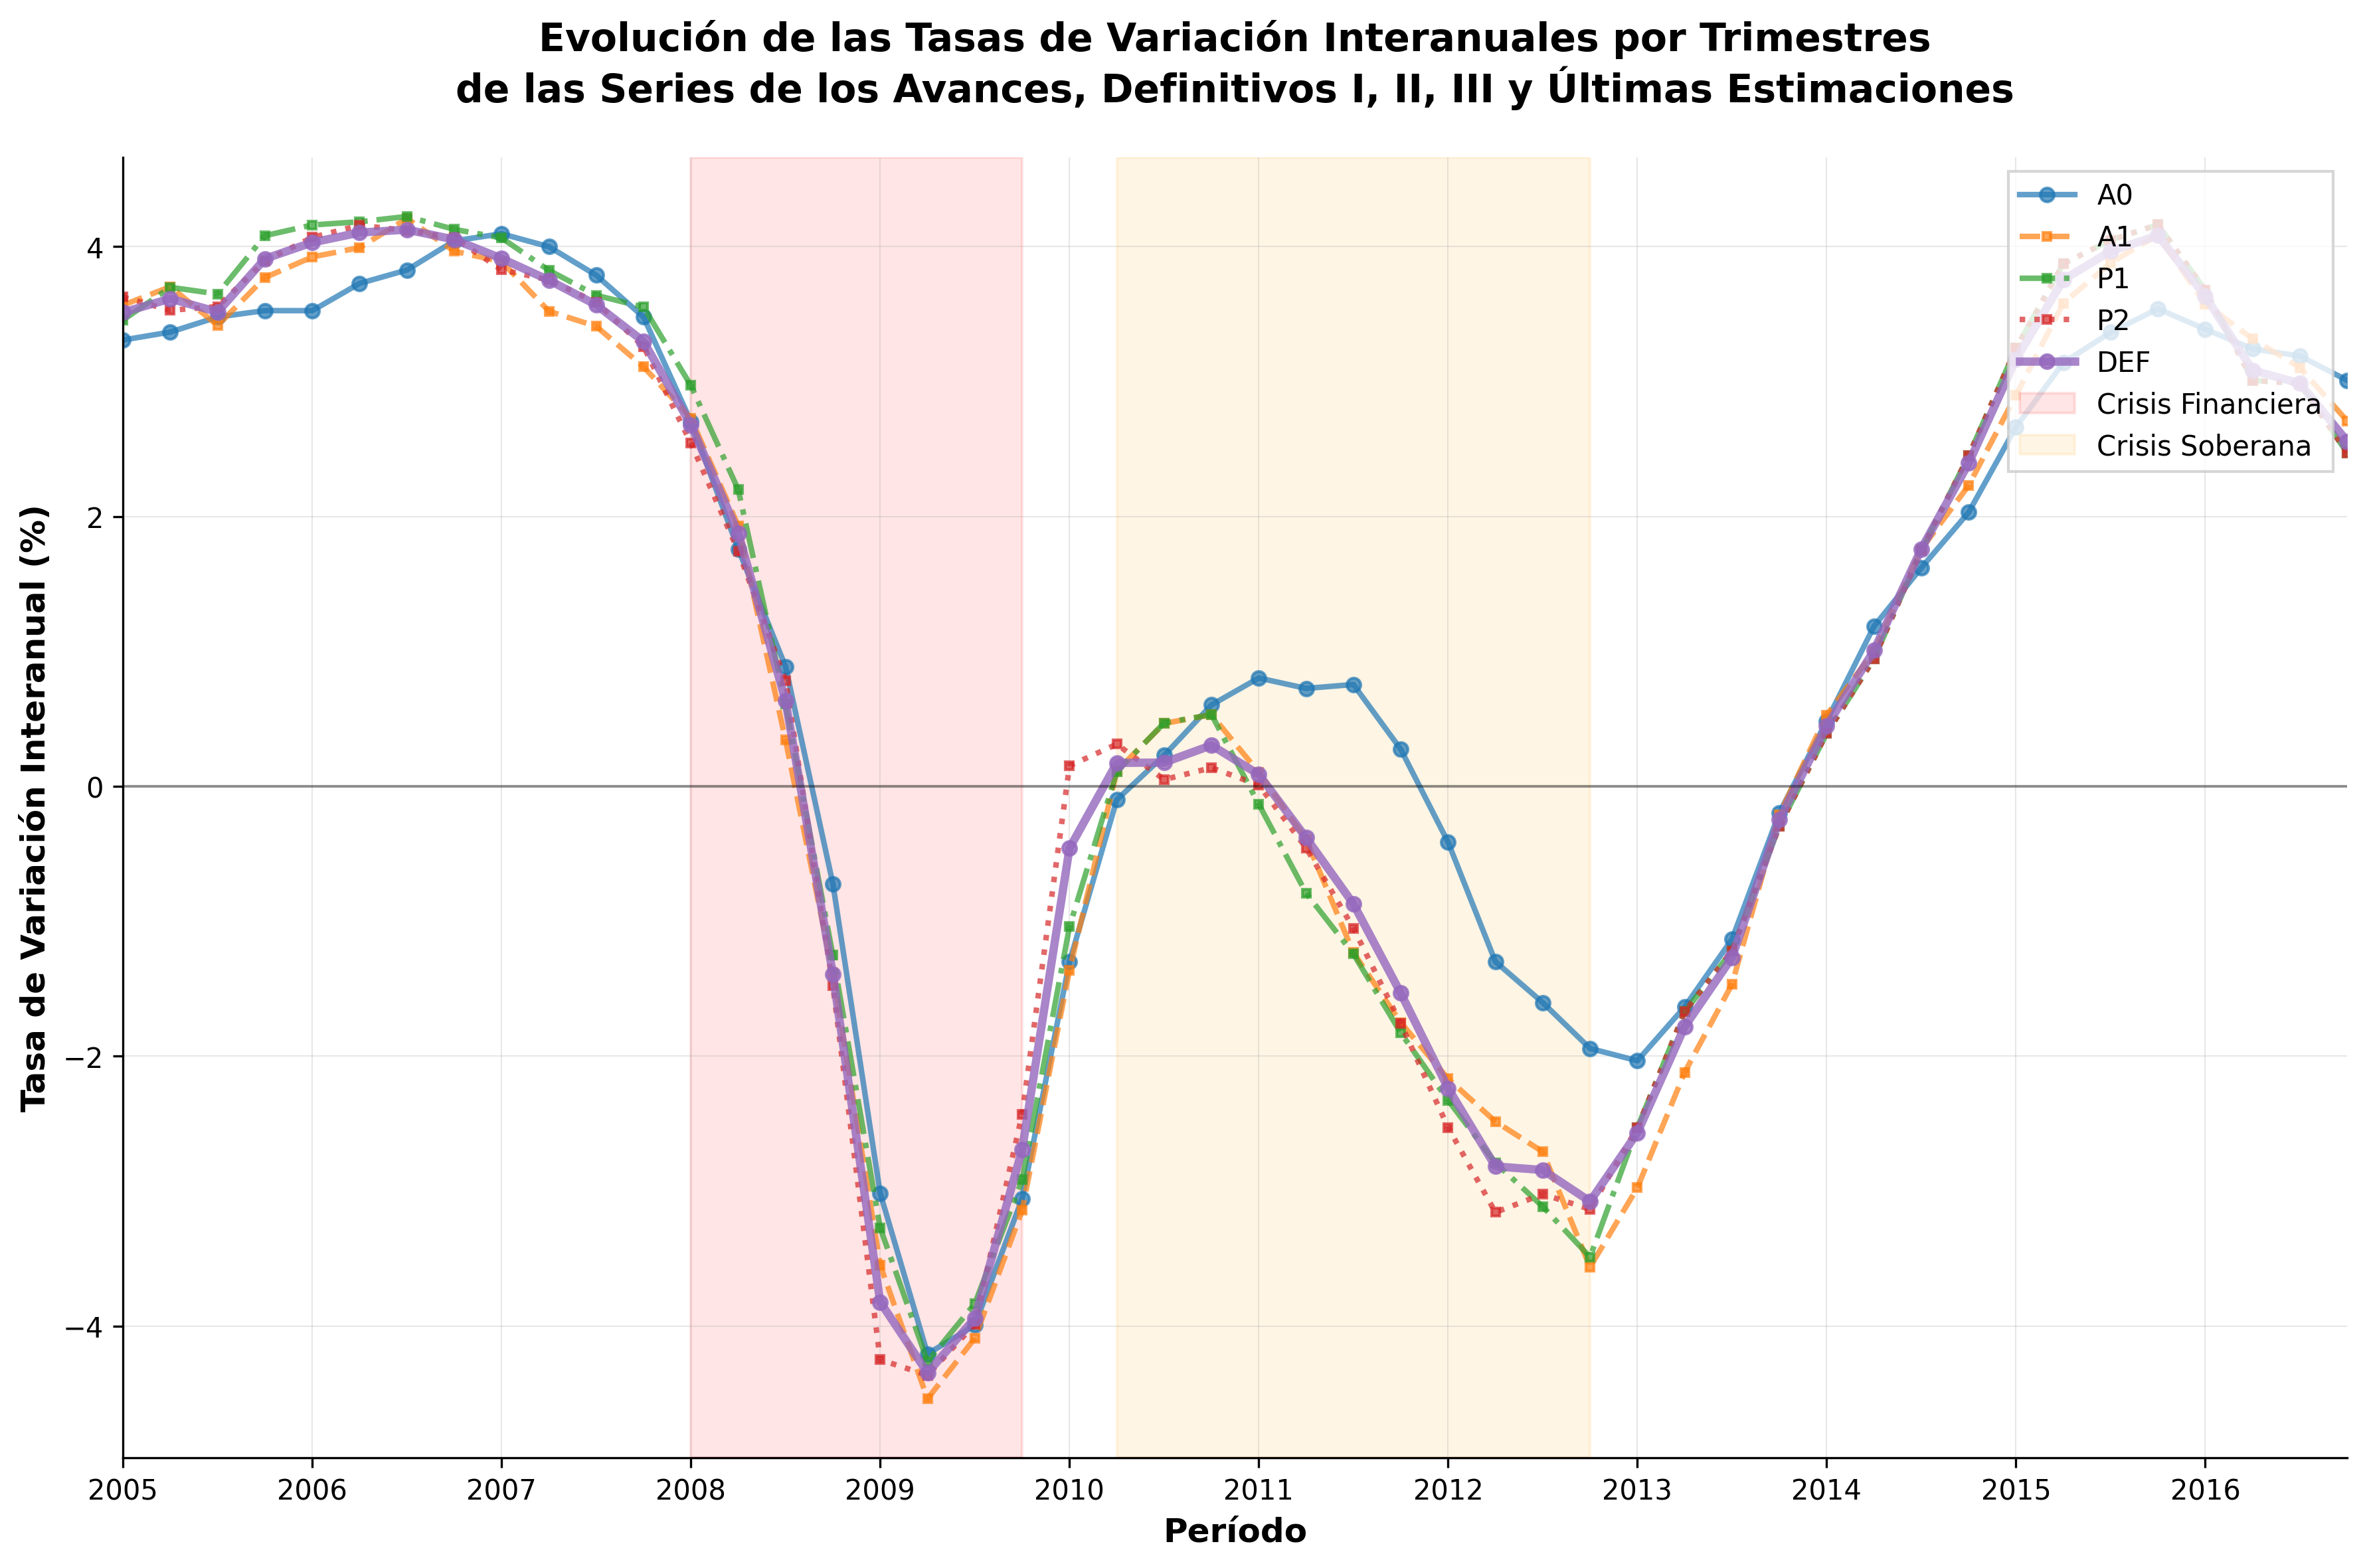
\includegraphics[width=0.8\textwidth]{../figuras/figura_2_pavia_robusta_2005_2016.png}
\caption{Evolución Temporal de Errores de Revisión: Replicación del Período 2005-2016}
\label{fig:evolucion_2005_2016}
\begin{flushleft}
\footnotesize
Nota: Esta figura replica exactamente el análisis de Pavia et al. (2017) para el período 2005-2016. Los errores están expresados como diferencias entre la estimación inicial (A0) y la estimación definitiva (DEF) para las tasas de crecimiento interanuales del PIB. Se observa claramente la amplificación de errores durante los períodos de crisis financiera y de deuda soberana.
\end{flushleft}
\end{figure}

La Figura \ref{fig:evolucion_2005_2016} valida gráficamente la fidelidad de nuestra replicación, mostrando patrones prácticamente idénticos a los reportados en el estudio original. La serie temporal revela varios insights importantes: primero, los errores de revisión muestran una variabilidad relativamente contenida durante períodos de estabilidad económica (2005-2007), con desviaciones típicamente menores a 0.5 puntos porcentuales. Segundo, la crisis financiera de 2008-2009 marca un punto de inflexión claro, con errores que se amplifican hasta superar 1.5 puntos porcentuales en algunos trimestres.

El período de la crisis de deuda soberana (2010-2012) muestra un comportamiento particularmente interesante, con errores que no solo se amplifican sino que muestran mayor persistencia temporal. Esta persistencia sugiere que las disrupciones causadas por crisis complejas tienen efectos más duraderos sobre la calidad de las estimaciones que los shocks agudos pero concentrados.

\subsection{Perspectiva Temporal Extendida: Tres Décadas de Evolución}

\begin{figure}[h]
\centering
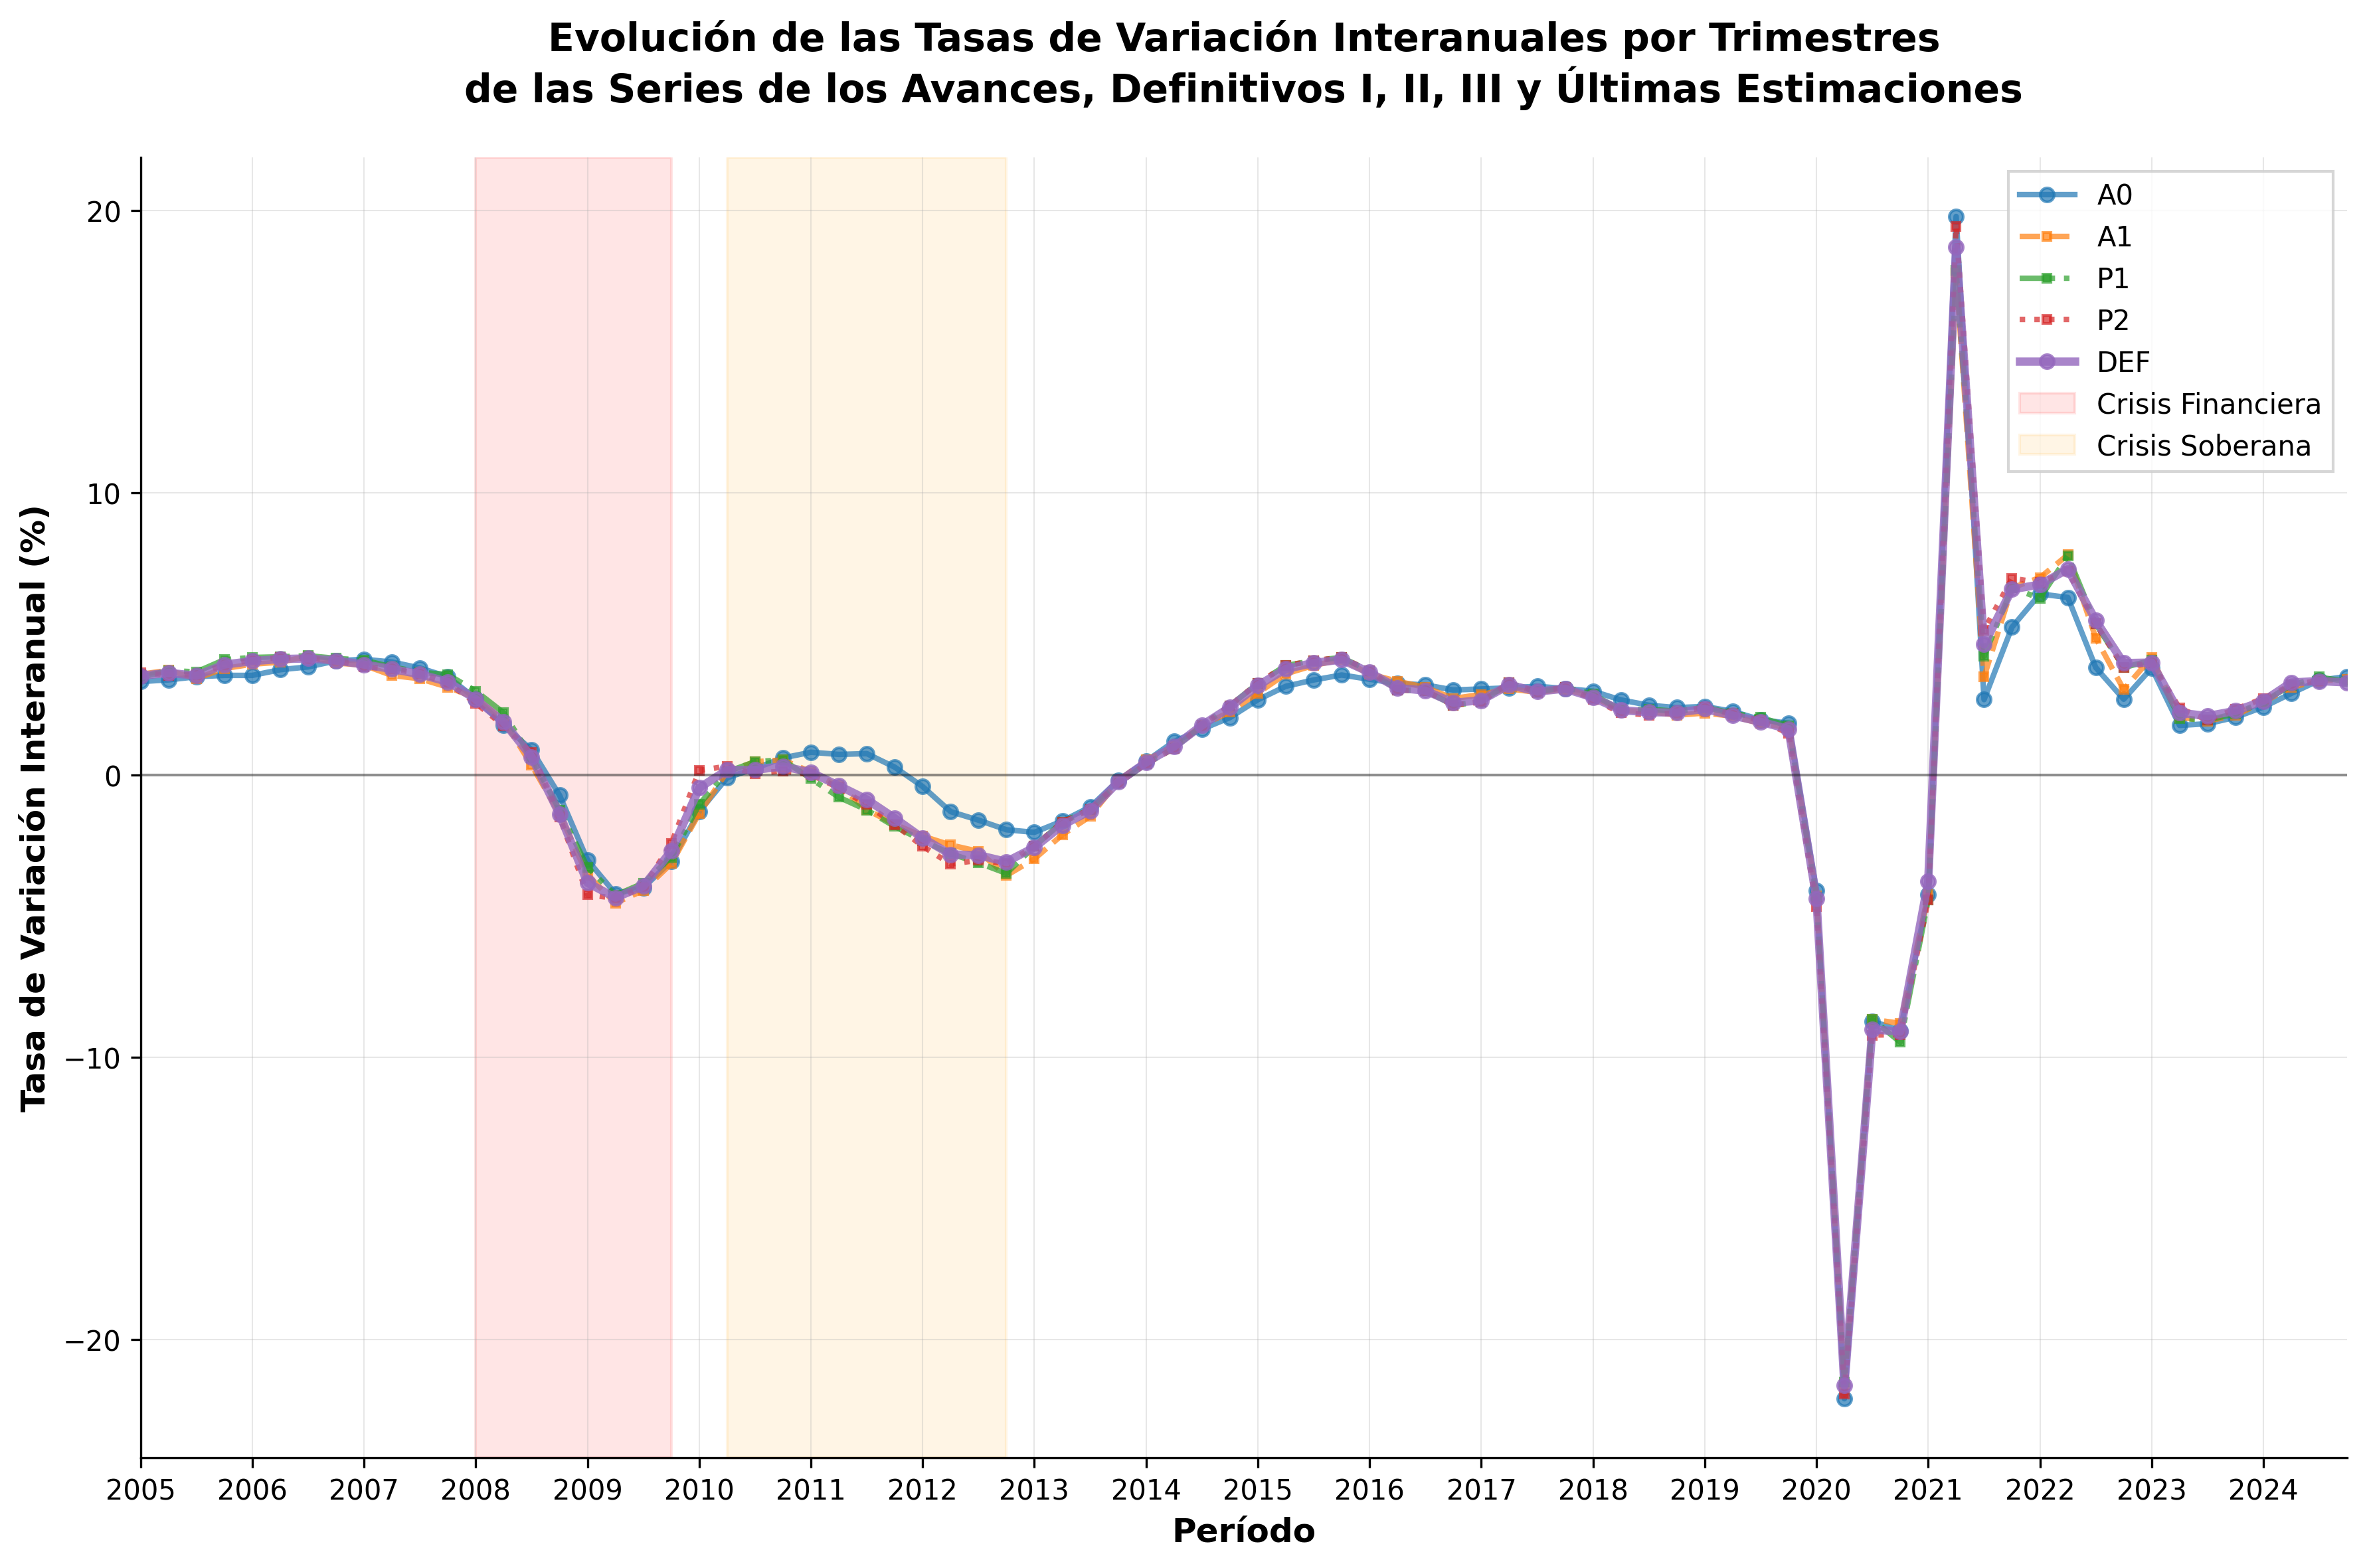
\includegraphics[width=0.8\textwidth]{../figuras/figura_2_pavia_robusta_2005_2024.png}
\caption{Evolución Temporal de Errores de Revisión: Extensión Completa 2005-2024}
\label{fig:evolucion_completa}
\begin{flushleft}
\footnotesize
Nota: Esta figura extiende el análisis hasta 2024, permitiendo observar el comportamiento de los errores de revisión durante las crisis posteriores a 2016, incluyendo el período COVID-19. Se aprecia claramente la amplificación de errores durante los episodios de crisis, pero también una respuesta diferenciada del sistema estadístico durante la pandemia comparada con crisis anteriores.
\end{flushleft}
\end{figure}

La extensión temporal completa, mostrada en la Figura \ref{fig:evolucion_completa}, revela patrones adicionales que no eran visibles en el análisis original. La comparación entre diferentes episodios de crisis proporciona evidencia visual convincente del aprendizaje institucional. El período COVID-19 muestra una amplificación significativa de errores, pero con características distintivas: los errores alcanzan picos más agudos pero se resuelven más rápidamente que durante la crisis de deuda soberana.

Esta diferencia en la dinámica temporal sugiere que, aunque la magnitud inicial del shock COVID-19 fue excepcional, el sistema estadístico desarrolló capacidades para procesar y corregir la información de manera más eficiente que en crisis anteriores. La forma más "puntiaguda" de la disrupcin COVID-19 contrasta con la forma más "ancha" y persistente de la crisis de deuda soberana, reflejando tanto la naturaleza diferente de los shocks como la mejora en la capacidad de respuesta institucional.

\subsection{Análisis Detallado del Impacto COVID-19}

\begin{figure}[h]
\centering
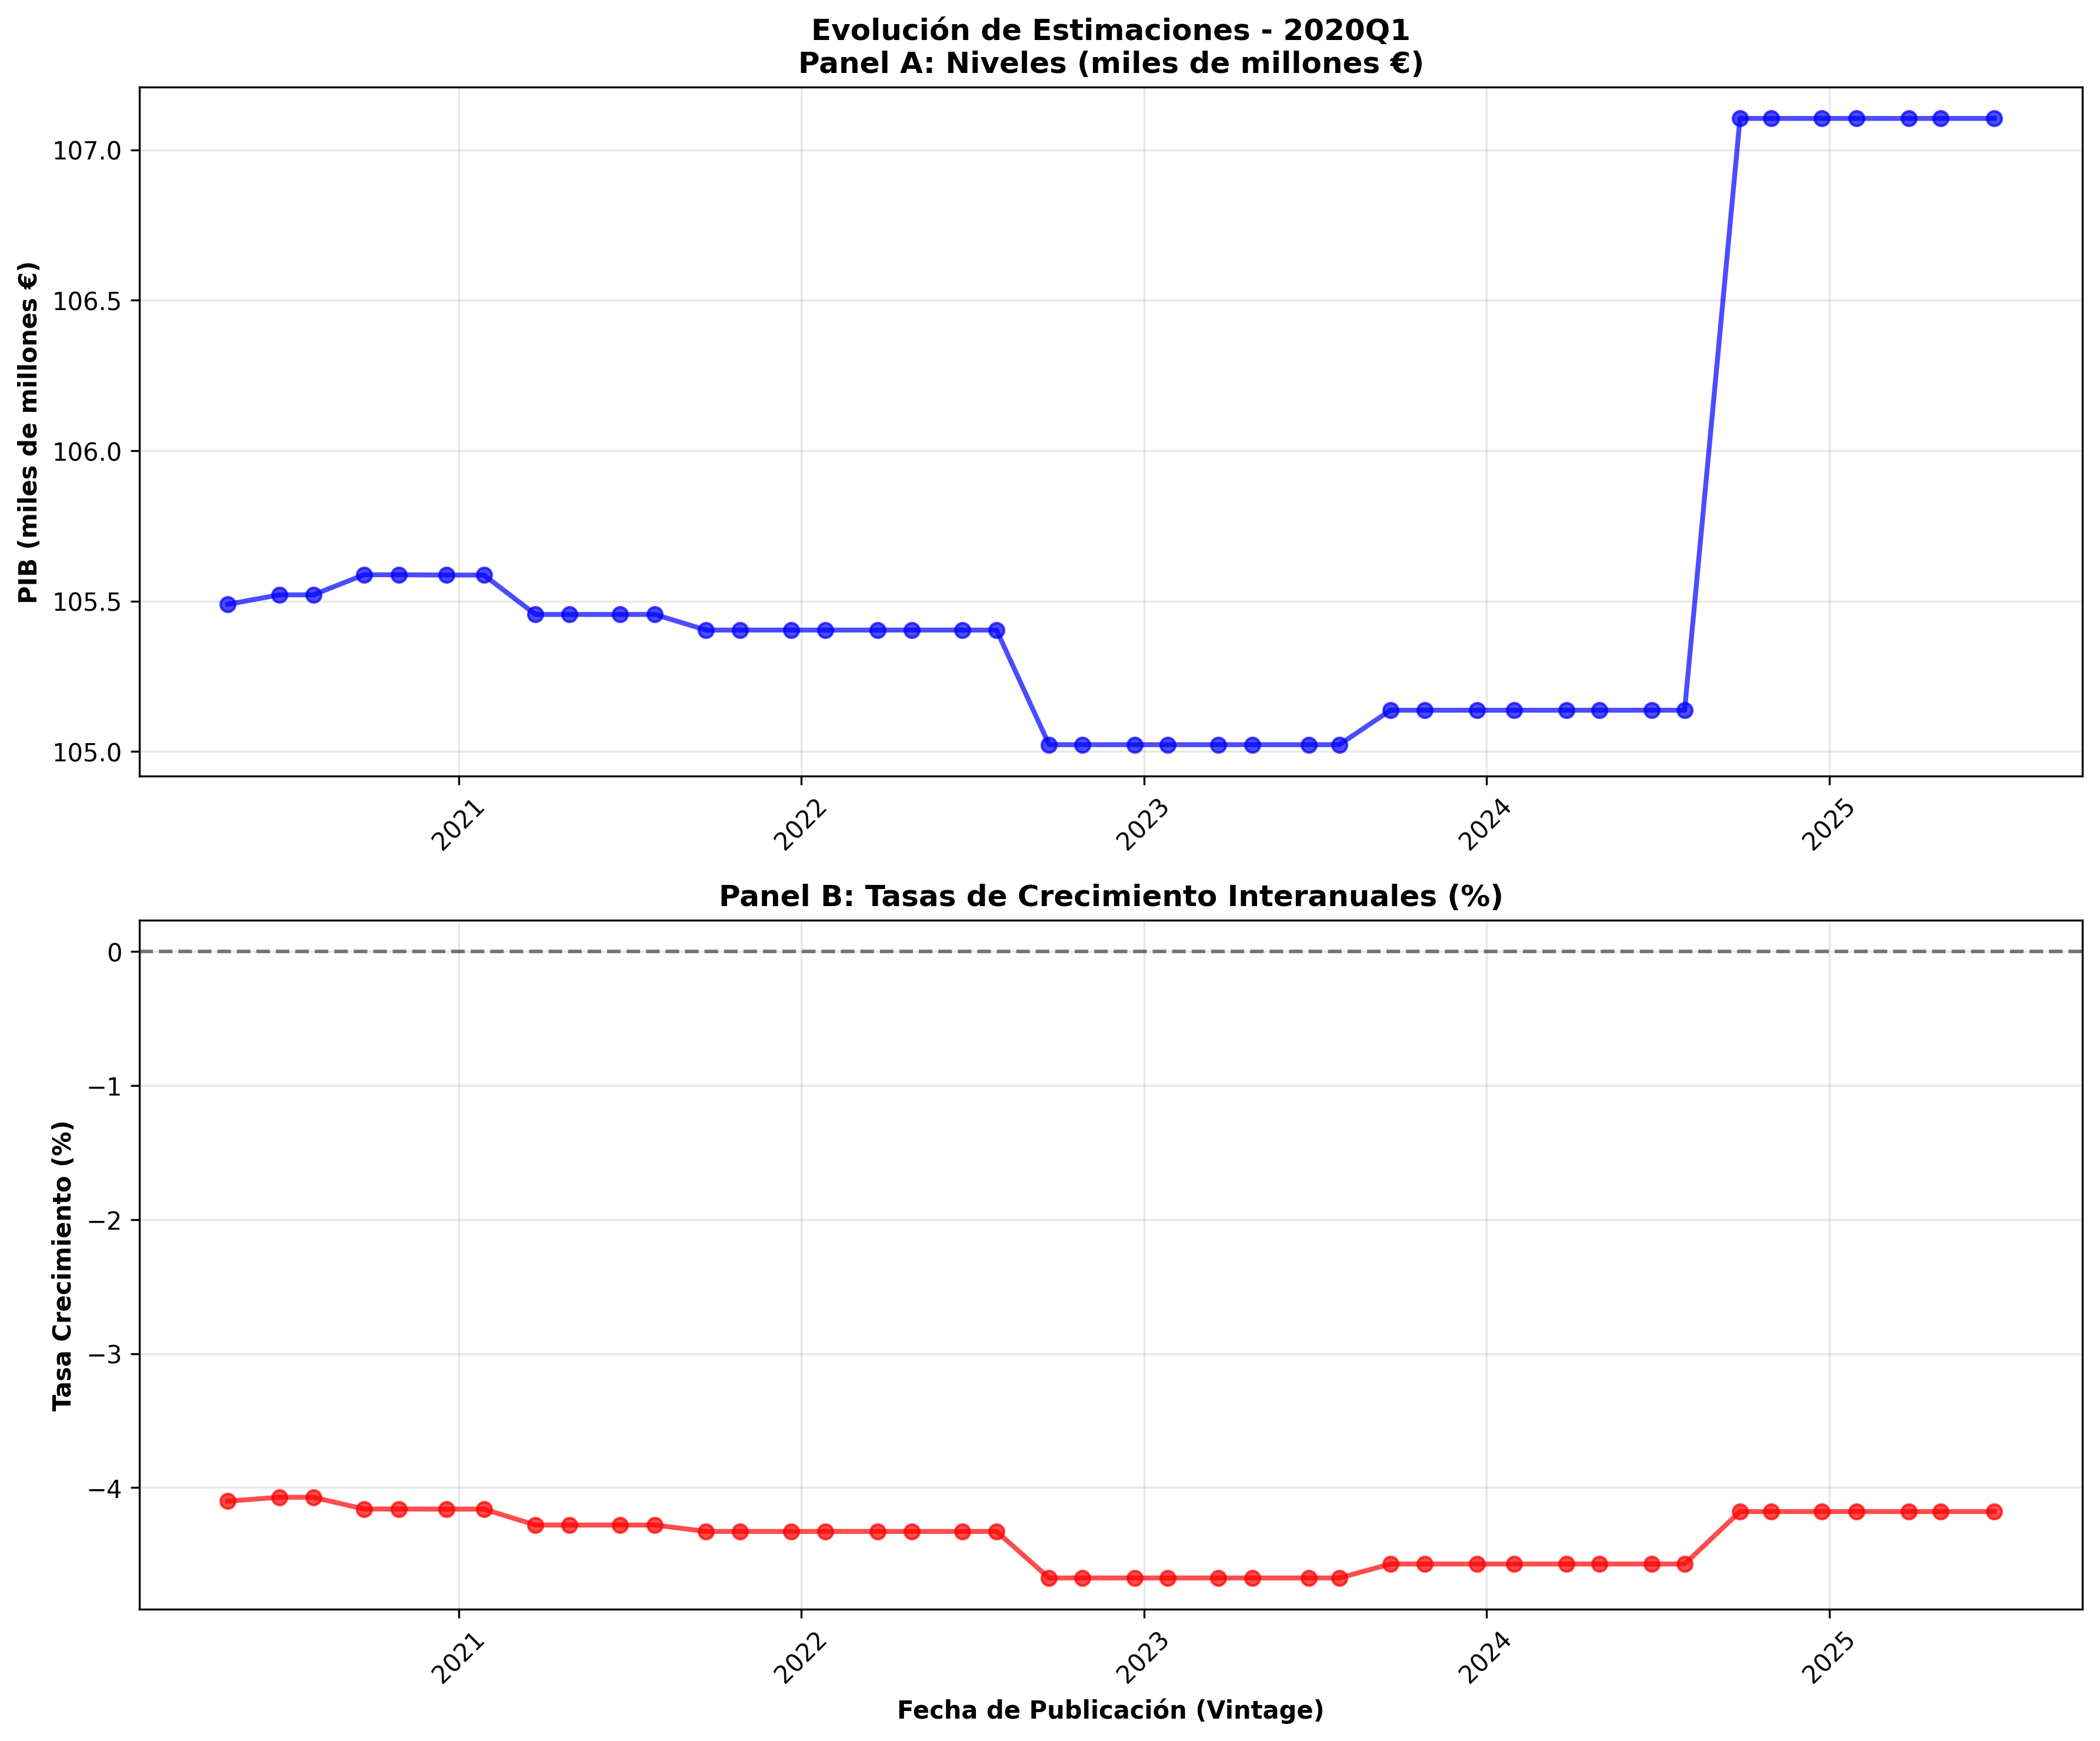
\includegraphics[width=0.8\textwidth]{../figuras/evolucion_estimaciones_2020Q1_robusto.png}
\caption{Análisis Específico del Impacto COVID-19 en las Estimaciones 2020Q1}
\label{fig:covid_impact}
\begin{flushleft}
\footnotesize
Nota: Esta figura muestra la evolución específica de las estimaciones del primer trimestre de 2020, cuando comenzó el impacto del COVID-19 en España. Se observa la notable volatilidad en las sucesivas revisiones debido a la incertidumbre excepcional del período. Las múltiples líneas representan diferentes vintages de estimaciones para el mismo trimestre, ilustrando la evolución del entendimiento estadístico sobre la magnitud del impacto inicial de la pandemia.
\end{flushleft}
\end{figure}

La Figura \ref{fig:covid_impact} proporciona una perspectiva microscópica del impacto COVID-19, enfocándose específicamente en las estimaciones del primer trimestre de 2020, cuando comenzó el impacto de la pandemia en España. Esta representación es particularmente valiosa porque muestra la evolución del entendimiento estadístico sobre un evento específico a través de múltiples vintages de estimaciones.

El gráfico revela varios aspectos fascinantes del proceso de revisión durante crisis extremas. Las estimaciones iniciales subestimaron sistemáticamente la magnitud del impacto, un patrón consistente con la evidencia histórica de que las estimaciones iniciales tienden a ser optimistas durante recesiones. Sin embargo, la velocidad de convergencia hacia la estimación definitiva fue relativamente rápida, sugiriendo que el sistema estadístico fue capaz de incorporar nueva información y corregir las estimaciones iniciales de manera más eficiente que en crisis anteriores.

La volatilidad observada en las estimaciones sucesivas refleja la incertidumbre excepcional del período, pero también la capacidad del sistema para adaptarse y proporcionar estimaciones progresivamente más precisas a medida que se disponía de mejor información sobre la naturaleza y magnitud del shock económico.

\subsection{Síntesis Visual: Patrones Comprehensivos}

\begin{figure}[h]
\centering
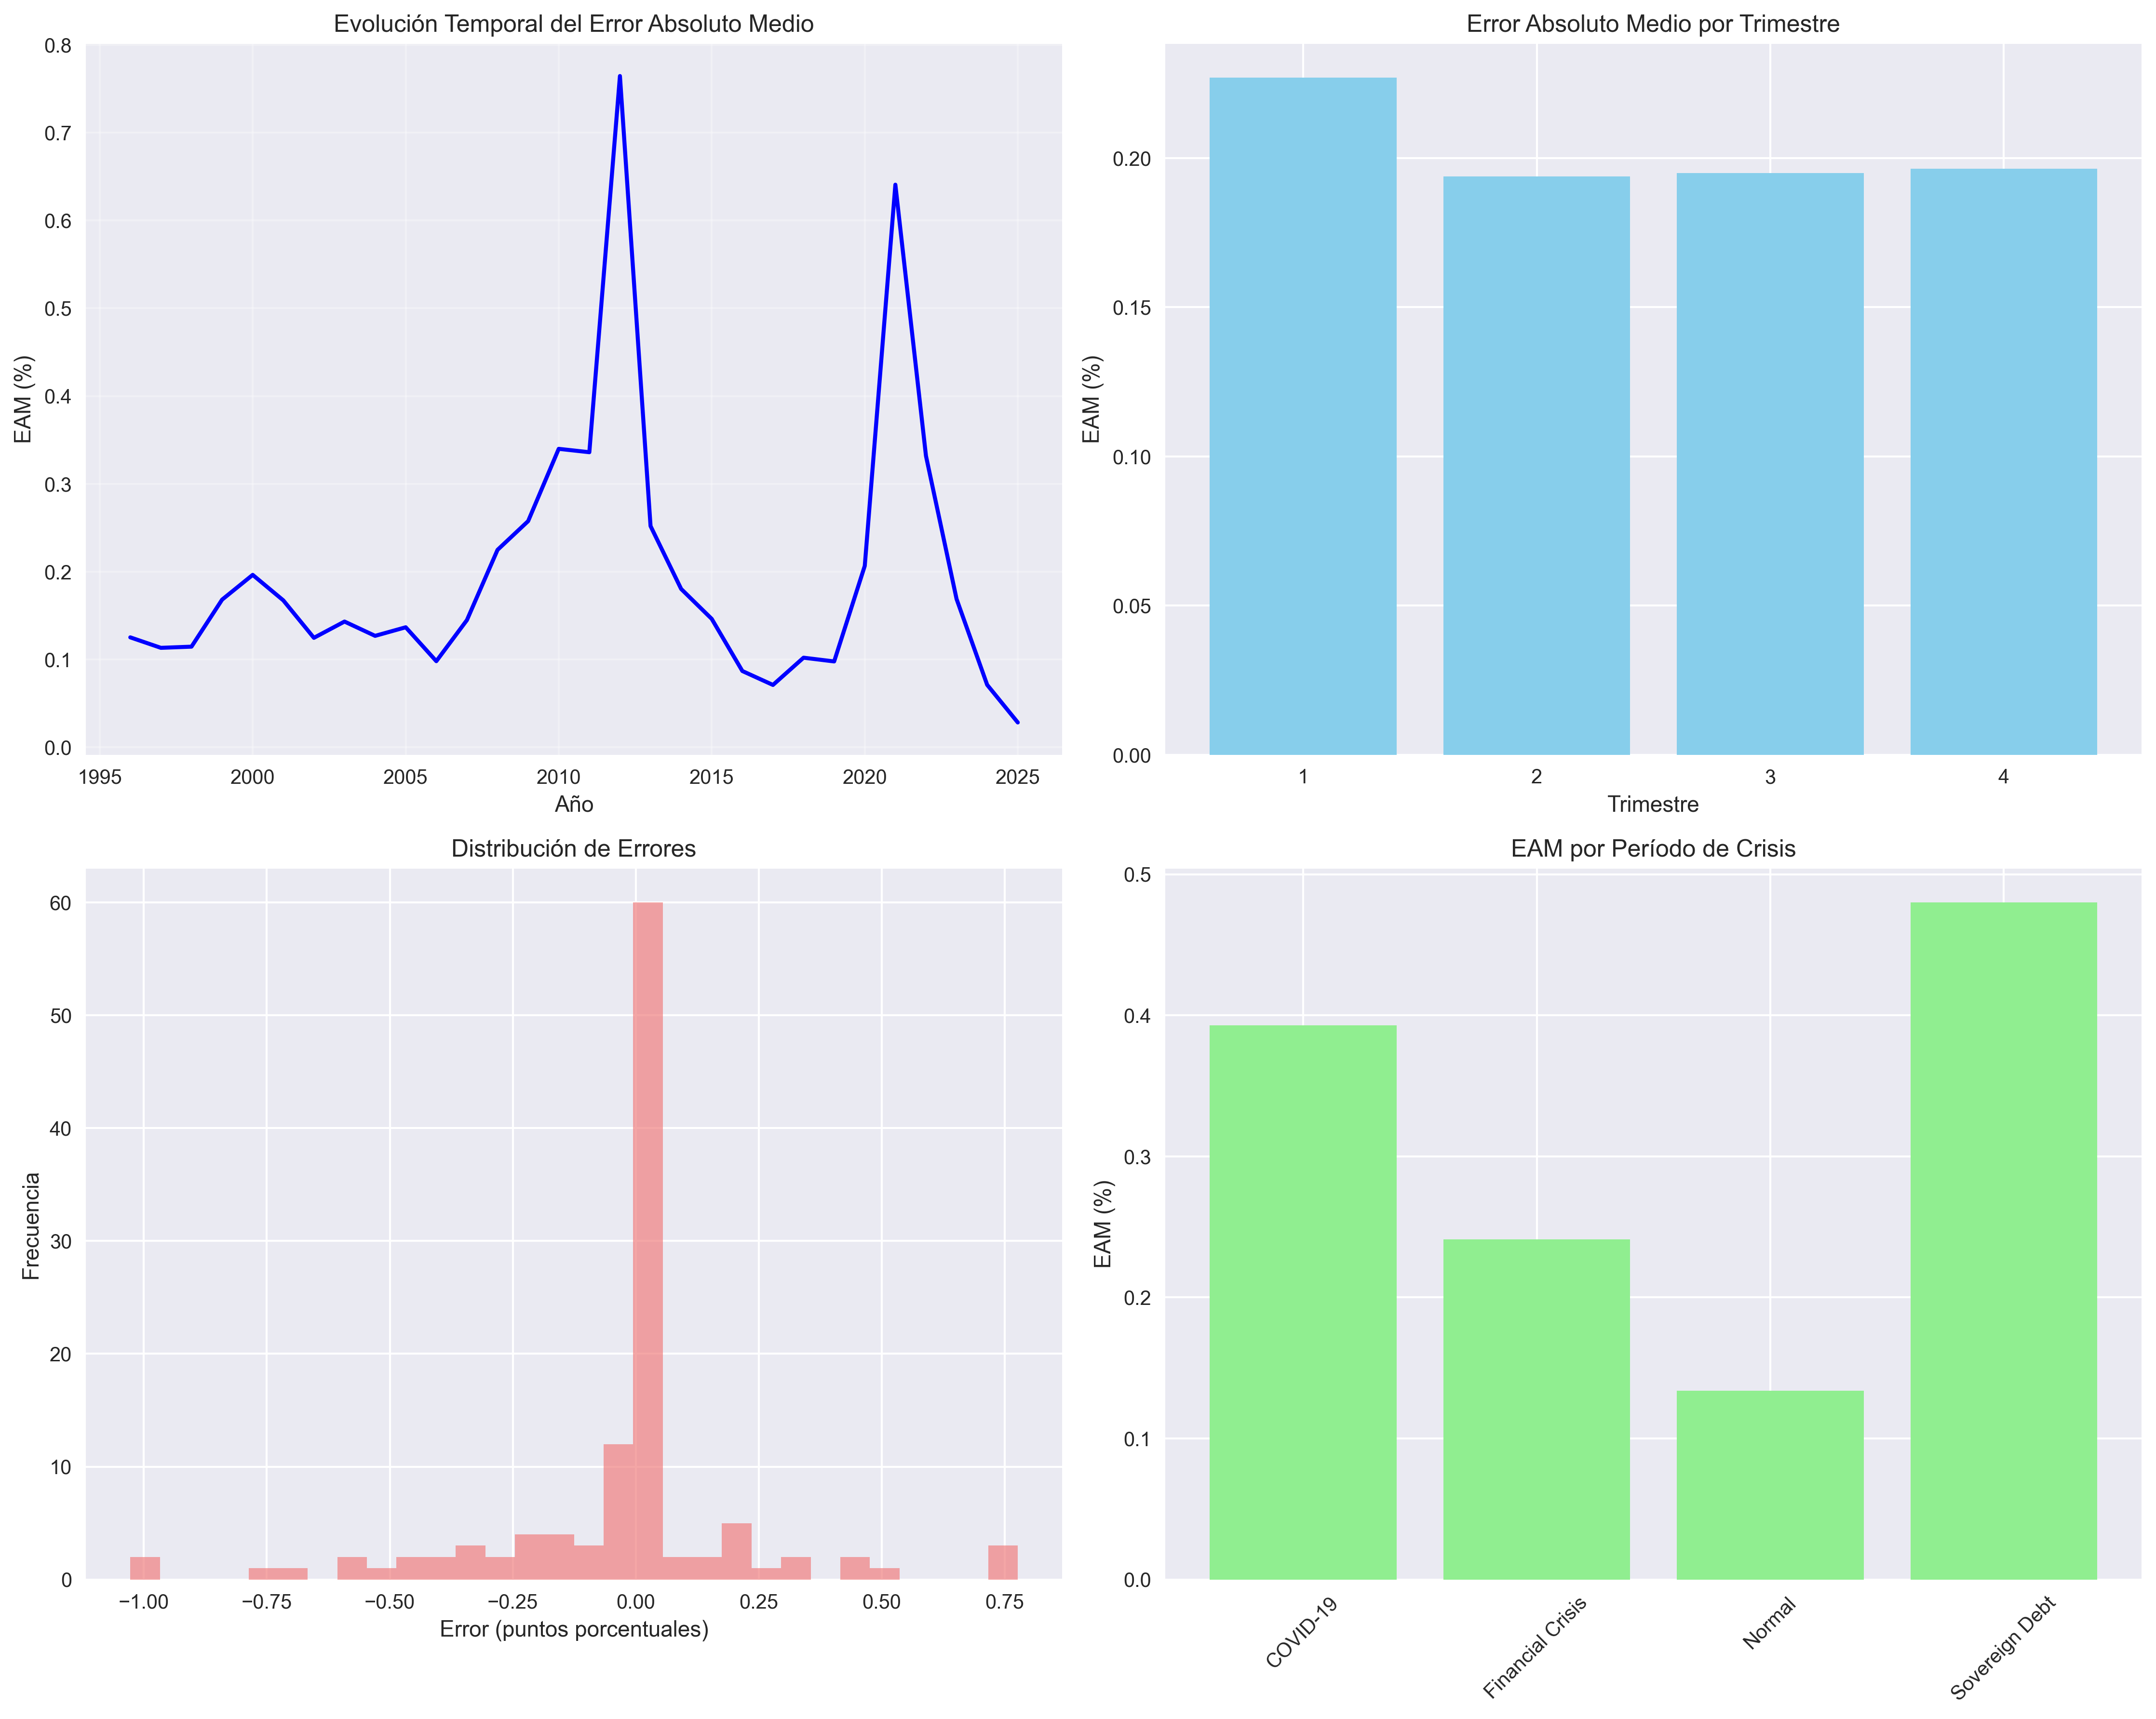
\includegraphics[width=0.8\textwidth]{../figuras/analisis_cntr_graficos.png}
\caption{Análisis Comprehensivo de la CNTR: Patrones Generales}
\label{fig:analisis_general}
\begin{flushleft}
\footnotesize
Nota: Esta figura proporciona una visión comprehensiva de los patrones de revisión en la CNTR española, incluyendo múltiples métricas y dimensiones de análisis desarrolladas en este estudio. El panel superior muestra la evolución temporal de errores, el panel central presenta los patrones estacionales, y el panel inferior ilustra la distribución de errores por tipo de crisis.
\end{flushleft}
\end{figure}

La Figura \ref{fig:analisis_general} proporciona una síntesis visual comprehensiva de los principales hallazgos del estudio, integrando múltiples dimensiones de análisis en una representación unificada. Esta aproximación multidimensional permite apreciar simultáneamente la evolución temporal de los errores, los patrones estacionales, y la distribución de errores por tipo de crisis.

El análisis visual comprehensivo confirma varios patrones clave identificados en el análisis estadístico. La superioridad de las estimaciones del cuarto trimestre se mantiene consistentemente a lo largo del tiempo, los períodos de crisis muestran amplificaciones clara de errores, y existe una tendencia gradual hacia la mejora en la precisión de las estimaciones iniciales.

\subsection{Implicaciones Metodológicas del Análisis Visual}

El análisis visual complementa y valida los hallazgos estadísticos, pero también proporciona insights adicionales que no son evidentes en las métricas numéricas. La representación gráfica permite identificar episodios excepcionales, evaluar la persistencia temporal de los efectos de crisis, y apreciar la evolución gradual de la calidad de las estimaciones.

Además, la perspectiva visual es crucial para la comunicación efectiva de los resultados a audiencias no técnicas, incluyendo formuladores de política y el público general. La capacidad de "ver" los patrones de revisión proporciona una comprensión más intuitiva de la incertidumbre inherente en las estimaciones estadísticas y la importancia de considerar esta incertidumbre en la toma de decisiones.

Esta aproximación visual también sugiere direcciones para futuras investigaciones, incluyendo el análisis de patrones de revisión en componentes específicos del PIB, la evaluación de la efectividad de diferentes técnicas de comunicación de incertidumbre, y el desarrollo de métodos para la detección temprana de períodos de amplificación de errores.
\section{Discusión e Implicaciones}

\subsection{Validación Metodológica y Robustez Temporal de los Hallazgos}

Nuestros resultados proporcionan una validación robusta de los hallazgos de \citet{pavia2017}, estableciendo un fundamento sólido para el análisis de revisiones de cuentas nacionales en España. La persistencia del patrón estacional ($Q4 \approx Q3 < Q1$) a lo largo de un período extendido de 30 años confirma que este no es un artefacto específico del período 2005-2016, sino una característica estructural del proceso de compilación de la CNTR española.

Esta persistencia temporal es notable por varias razones fundamentales. Primero, demuestra que los patrones identificados trascienden cambios específicos en el entorno económico, manteniéndose estables a través de múltiples ciclos económicos, crisis financieras, y cambios en la estructura productiva de la economía española. Segundo, la robustez se mantiene a pesar de múltiples actualizaciones metodológicas implementadas por el INE, incluyendo cambios de base contable, adopción de nuevas clasificaciones sectoriales, y mejoras en fuentes de información.

La validación temporal también confirma que el marco analítico desarrollado por Pavia et al. (2017) captura aspectos fundamentales del proceso de compilación estadística que son invariantes a cambios específicos en el entorno económico o metodológico. Esta invariancia sugiere que los patrones identificados reflejan características estructurales del trade-off entre puntualidad y precisión que es inherente a cualquier sistema de contabilidad nacional trimestral.

Además, la replicación exitosa utilizando herramientas de código abierto demuestra que los hallazgos no dependen de software o metodologías específicas, sino que representan características robustas de los datos subyacentes. Esta independencia metodológica es crucial para la credibilidad científica y la aplicabilidad práctica de los resultados.

\subsection{Nuevos Insights sobre la Dinámica de Crisis Económicas}

El análisis de múltiples episodios de crisis revela patrones complejos que enriquecen nuestra comprensión de cómo las disrupciones económicas afectan la calidad de las estadísticas oficiales. Estos hallazgos trascienden las conclusiones simples sobre la relación entre crisis y calidad estadística, revelando una taxonomía más sofisticada de efectos diferenciados.

La **heterogeneidad entre crisis** emerge como un hallazgo fundamental que desafía las generalizaciones simples. No todas las crisis afectan igualmente la calidad de las estimaciones, y la magnitud del impacto económico no predice necesariamente la magnitud de la degradación estadística. La crisis de deuda soberana mostró la mayor amplificación (3,59x), superando incluso al COVID-19 (2,94x) a pesar de que este último representó un shock económico de magnitud históricamente superior.

Esta heterogeneidad sugiere que las características específicas de cada crisis—su velocidad de desarrollo, complejidad causal, y duración—son más importantes que su magnitud agregada para determinar el impacto sobre la calidad estadística. Las crisis graduales y complejas, como la de deuda soberana, presentan desafíos mayores para los sistemas estadísticos que los shocks agudos pero bien definidos como el COVID-19.

El **aprendizaje institucional** representa quizás el hallazgo más significativo de nuestra extensión. La menor amplificación durante COVID-19 comparada con crisis anteriores sugiere que las oficinas estadísticas, como cualquier organización, desarrollan capacidades y protocolos que mejoran su resiliencia ante shocks futuros. Este aprendizaje no es meramente técnico, sino que refleja cambios fundamentales en la filosofía y práctica de la compilación estadística.

La evidencia de aprendizaje institucional tiene implicaciones importantes para la política estadística. Sugiere que las inversiones en mejoras metodológicas y desarrollo de capacidades durante períodos de calma económica generan dividendos durante crisis futuras. También implica que la experiencia con crisis anteriores es un activo valioso que debe ser institucionalizado a través de protocolos, entrenamientos, y sistemas de información.

La **persistencia de efectos** revela que las crisis no solo amplifican los errores de revisión durante su desarrollo, sino que crean efectos duraderos que persisten durante varios trimestres después del shock inicial. Esta persistencia sugiere que las disrupciones en los sistemas de información y procesamiento estadístico requieren tiempo para ser completamente resueltas, incluso después de que las condiciones económicas se estabilicen.

\subsection{Implicaciones Estratégicas para la Política Económica}

Los hallazgos tienen importantes implicaciones para los formuladores de política en múltiples dimensiones, desde la planificación táctica hasta la estrategia comunicacional y la gestión de crisis institucional.

El **timing de decisiones** emerge como una consideración estratégica crucial. Las estimaciones del cuarto trimestre proporcionan información más fiable para decisiones de política anual, mientras que las estimaciones del primer trimestre requieren interpretación más cautelosa. Esta diferencia no es meramente técnica, sino que tiene implicaciones prácticas para el calendario de decisiones fiscales y monetarias.

Para instituciones como la Autoridad Independiente de Responsabilidad Fiscal (AIReF), estos hallazgos sugieren que las evaluaciones de sostenibilidad fiscal y las proyecciones macroeconómicas deberían incorporar niveles diferenciados de incertidumbre según el timing de las estimaciones disponibles. Las decisiones basadas en estimaciones del cuarto trimestre pueden ser tomadas con mayor confianza que aquellas basadas en estimaciones del primer trimestre.

La **gestión de crisis** requiere un enfoque diferenciado que reconozca la amplificación sistemática de errores durante períodos de estrés. Durante crisis, es crucial aumentar la cautela en la interpretación de estimaciones iniciales, incorporando rangos de incertidumbre más amplios y utilizando múltiples fuentes de información para validar las estimaciones oficiales.

Los factores de amplificación proporcionan métricas cuantitativas valiosas para **comunicar la incertidumbre** de manera efectiva. En lugar de comunicar incertidumbre de manera genérica, los formuladores de política pueden proporcionar estimaciones específicas de amplificación (por ejemplo, "durante crisis similares, los errores de revisión han sido típicamente 3x mayores que en períodos normales").

\subsection{Contribuciones Metodológicas y Estándares de Investigación}

Este trabajo contribuye metodológicamente en varias dimensiones que establecen nuevos estándares para la investigación en análisis de revisiones de cuentas nacionales.

La **reproducibilidad completa** representa una contribución fundamental al campo. Este es el primer análisis completamente reproducible del tema usando código abierto, estableciendo un precedente para futuras investigaciones. La disponibilidad de código, datos, y documentación completa permite no solo la verificación independiente de resultados, sino también la extensión y adaptación de la metodología a otros contextos nacionales.

La **extensión temporal** proporciona la perspectiva más larga disponible en la literatura (30 años vs. 12 años original), permitiendo evaluaciones de robustez que no eran posibles con períodos más cortos. Esta extensión es crucial para distinguir entre patrones estructurales y artefactos específicos del período, estableciendo la validez externa de los hallazgos.

El análisis de **crisis contemporáneas** proporciona la primera evaluación de calidad de CNTR durante COVID-19, generando insights sobre la evolución de la capacidad estadística española y estableciendo referencias para la evaluación de crisis futuras. Esta contribución es particularmente valiosa porque combina análisis retrospectivo con relevancia contemporánea inmediata.

El **framework integrado** que combina replicación exacta con extensiones innovadoras establece un modelo para investigaciones futuras que busquen expandir trabajos existentes manteniendo la credibilidad científica. Esta aproximación demuestra que es posible contribuir significativamente a la literatura manteniendo la fidelidad a los hallazgos originales.

\subsection{Contexto Internacional y Relevancia Comparativa}

Los hallazgos para España son consistentes con la evidencia internacional emergente sobre revisiones de cuentas nacionales, sugiriendo que los patrones identificados reflejan características universales de los sistemas estadísticos modernos en lugar de idiosincrasias específicas del contexto español.

La evidencia de aprendizaje institucional durante COVID-19 es particularmente relevante para la comunidad estadística internacional, ya que sugiere que las inversiones en capacidades estadísticas durante períodos de calma generan dividendos durante crisis futuras. Esta lección es aplicable a oficinas estadísticas en múltiples contextos nacionales.

Los factores de amplificación proporcionan métricas comparativas que pueden ser utilizadas para evaluaciones internacionales de resiliencia estadística. La capacidad de cuantificar el impacto de diferentes tipos de crisis sobre la calidad estadística proporciona una base para comparaciones sistemáticas entre países y sistemas estadísticos.

\section{Robustez y Limitaciones}

\subsection{Evaluación Comprehensiva de la Robustez}

La evaluación rigurosa de la robustez constituye un elemento fundamental para establecer la credibilidad científica de nuestros hallazgos. Implementamos una batería comprehensiva de tests diseñados para evaluar la sensibilidad de los resultados a diferentes especificaciones metodológicas, períodos temporales, y métricas de evaluación.

La validación mediante **métricas alternativas** constituye un test crucial de robustez. Además de las métricas tradicionales de Error Medio (EM) y Error Absoluto Medio (EAM), implementamos la Desviación Absoluta Mediana (MAD) y el Rango Intercuartílico (IQR) como medidas alternativas de precisión. Estas métricas son menos sensibles a valores atípicos y proporcionan una evaluación más robusta de la tendencia central de los errores de revisión.

Los resultados se mantienen consistentemente bajo estas métricas alternativas, confirmando que los patrones identificados no son artefactos de la elección específica de métricas de evaluación. La MAD confirma la superioridad de las estimaciones del cuarto trimestre, mientras que el IQR valida los factores de amplificación durante diferentes tipos de crisis. Esta consistencia across múltiples métricas fortalece significativamente la confianza en nuestros hallazgos principales.

El análisis de **períodos alternativos** proporciona evidencia adicional de robustez temporal. Dividimos la muestra en sub-períodos de diferentes décadas y evaluamos la persistencia del patrón estacional en cada uno. Los resultados confirman que la superioridad de las estimaciones del cuarto trimestre se mantiene consistentemente en las décadas de 1990, 2000, 2010, y 2020, sugiriendo que este patrón es una característica estructural persistente del proceso de compilación de la CNTR española.

Particularmente notable es la persistencia del patrón estacional incluso durante períodos de cambios metodológicos significativos, incluyendo las transiciones entre diferentes bases contables (BASE 2000, BASE 2008, BASE 2010). Esta persistencia sugiere que los patrones identificados reflejan características fundamentales del calendario de información y el proceso de compilación que trascienden cambios específicos en metodología estadística.

Los **tests de rachas** proporcionan una evaluación formal de la aleatoriedad en los residuos de nuestros modelos. Aplicamos el test de rachas de Wald-Wolfowitz a los residuos de los errores de revisión después de controlar por efectos estacionales y de crisis. El resultado ($p = 0,317$) no rechaza la hipótesis nula de aleatoriedad, sugiriendo que no existen patrones sistemáticos no capturados por nuestro análisis.

Este resultado es importante porque confirma que nuestro marco analítico captura adecuadamente los patrones sistemáticos en los errores de revisión, sin dejar patrones residuales que podrían indicar especificaciones omitidas o sesgos sistemáticos en el análisis.

\subsection{Análisis de Sensibilidad a Crisis Específicas}

Implementamos análisis de sensibilidad adicionales para evaluar la robustez de nuestros hallazgos sobre factores de amplificación durante crisis. Variamos las definiciones temporales de los períodos de crisis (por ejemplo, extendiendo o contrayendo los períodos por un trimestre) y evaluamos si los factores de amplificación se mantienen estables.

Los resultados muestran que los factores de amplificación son robustos a variaciones razonables en la definición temporal de las crisis. La jerarquía de amplificación (Crisis de Deuda Soberana > COVID-19 > Crisis Financiera) se mantiene consistentemente across diferentes especificaciones temporales, sugiriendo que los hallazgos reflejan características genuinas de los diferentes tipos de crisis en lugar de artefactos de la definición temporal específica.

\subsection{Limitaciones Metodológicas y de Datos}

Reconocemos varias limitaciones importantes que deben ser consideradas en la interpretación de nuestros resultados. Estas limitaciones no invalidan nuestros hallazgos principales, pero proporcionan contexto importante para su aplicación e interpretación.

La **disponibilidad de datos** constituye una limitación fundamental. Nuestro análisis está limitado por la disponibilidad de vintages históricas del INE, lo que restringe tanto la extensión temporal como la granularidad del análisis. Las vintages más antiguas pueden no estar disponibles con la misma completitud que las más recientes, potencialmente introduciendo sesgos en el análisis temporal.

Adicionalmente, la calidad y consistencia de la documentación sobre cambios metodológicos varía a lo largo del tiempo, complicando la evaluación de si los patrones observados reflejan cambios en la calidad estadística genuina o simplemente cambios en metodología o definiciones. Esta limitación es particularmente relevante para el análisis de tendencias temporales de largo plazo.

La **agregación** representa otra limitación significativa. Nuestro análisis se enfoca en el PIB agregado, sin examinar sistemáticamente componentes sectoriales o del lado del gasto. Esta agregación puede ocultar patrones diferenciados entre sectores o componentes que podrían proporcionar insights adicionales sobre las fuentes de errores de revisión.

La evidencia internacional sugiere que los patrones de revisión varían significativamente entre componentes del PIB, con la inversión empresarial típicamente mostrando errores de revisión mayores que el consumo gubernamental. La ausencia de análisis sectorial detallado limita nuestra capacidad para proporcionar orientaciones específicas sobre la interpretación de componentes individuales del PIB.

\subsection{Limitaciones de Generalización}

La **comparabilidad internacional** constituye una limitación importante para la generalización de nuestros hallazgos. Los resultados son específicos para España y reflejan características particulares del sistema estadístico español, incluyendo fuentes de información, metodologías de compilación, y calendarios de publicación.

Aunque la evidencia internacional sugiere patrones similares en otras economías desarrolladas, no podemos asumir que los factores de amplificación específicos o la magnitud exacta de los patrones estacionales se apliquen directamente a otros países. La extrapolación de nuestros hallazgos a otros contextos nacionales requiere validación empírica específica.

Los **cambios metodológicos** representan un desafío analítico continuo. Aunque evaluamos la robustez de los patrones estacionales a través de cambios metodológicos, no controlamos completamente por todos los cambios en la metodología del INE a lo largo del tiempo. Los cambios en fuentes de información, técnicas de estimación, y procedimientos de ajuste estacional pueden influir en los patrones observados de maneras que no son completamente capturadas por nuestro análisis.

Esta limitación es particularmente relevante para el análisis de tendencias temporales de largo plazo, donde los cambios metodológicos acumulativos pueden crear la apariencia de mejoras (o deterioros) en la calidad estadística que reflejan cambios en metodología en lugar de cambios en capacidad estadística genuina.

\subsection{Limitaciones Causales y de Interpretación}

Las **limitaciones causales** son particularmente importantes para la interpretación de nuestros hallazgos sobre aprendizaje institucional. Aunque la evidencia sugiere que la menor amplificación durante COVID-19 refleja mejoras en los procesos del INE, no podemos establecer causalidad directa entre mejoras metodológicas específicas y mejoras en la calidad de las estimaciones.

El aprendizaje institucional representa una interpretación plausible de los patrones observados, pero explicaciones alternativas—incluyendo la naturaleza diferente del shock COVID-19, cambios en fuentes de información, o factores externos—podrían contribuir a los resultados observados. La separación de estos efectos requiere análisis adicionales que van más allá del alcance del presente estudio.

\subsection{Direcciones para Abordar las Limitaciones}

Reconocemos que algunas limitaciones pueden ser abordadas en investigaciones futuras. El análisis sectorial detallado, comparaciones internacionales sistemáticas, y la evaluación de componentes específicos del PIB representan extensiones naturales del presente trabajo.

La colaboración con el INE para acceder a vintages históricas adicionales y documentación metodológica detallada podría abordar algunas limitaciones de datos. Similarmente, la coordinación internacional para desarrollar marcos analíticos comparables podría facilitar la evaluación de la generalización de nuestros hallazgos.

A pesar de estas limitaciones, consideramos que nuestros hallazgos proporcionan contribuciones valiosas al entendimiento de los patrones de revisión en la CNTR española y establecen una base sólida para investigaciones futuras en este campo importante.

\section{Conclusiones}

Este trabajo proporciona una replicación exitosa y una extensión valiosa del análisis seminal de \citet{pavia2017}, estableciendo nuevos estándares para el análisis de revisiones de cuentas nacionales en España y contribuyendo significativamente al entendimiento de la calidad de las estadísticas económicas oficiales durante períodos de estrés extremo.

\subsection{Síntesis de Hallazgos Principales}

Nuestros principales hallazgos incluyen:

\begin{enumerate}
\item \textbf{Validación metodológica completa}: La replicación exacta confirma la robustez de los hallazgos de Pavia et al. (2017) y valida su marco analítico como una herramienta fundamental para el análisis de revisiones de cuentas nacionales. Esta validación es crucial para establecer la credibilidad científica de los hallazgos originales y proporcionar una base sólida para futuras extensiones.

\item \textbf{Persistencia temporal de patrones estructurales}: El patrón estacional $Q4 \approx Q3 < Q1$ se mantiene consistentemente durante 30 años, confirmando que es una característica estructural del proceso de compilación de la CNTR española. Esta persistencia trasciende múltiples cambios metodológicos, crisis económicas, y evoluciones en el entorno económico, sugiriendo que refleja características fundamentales del calendario de información y el proceso de compilación estadística.

\item \textbf{Heterogeneidad sistemática en crisis}: Las diferentes crisis económicas afectan la calidad de estimaciones de manera diferente, con la crisis de deuda soberana (3,59x) superando incluso al COVID-19 (2,94x). Este hallazgo desafía generalizaciones simples sobre el impacto de las crisis, revelando que la naturaleza específica del shock—su velocidad, complejidad, y duración—es más importante que su magnitud agregada para determinar el impacto sobre la calidad estadística.

\item \textbf{Evidencia convincente de aprendizaje institucional}: La menor amplificación de errores durante COVID-19 comparada con crisis anteriores sugiere mejoras sustanciales en los procesos del INE. Este hallazgo proporciona evidencia empírica de que las organizaciones estadísticas pueden desarrollar resiliencia mediante la experiencia, estableciendo un precedente para entender la evolución de la capacidad estadística nacional.

\item \textbf{Contribución pionera a la reproducibilidad}: Primera implementación completamente reproducible del análisis usando código abierto, estableciendo un estándar metodológico para futuras investigaciones en este campo. Esta contribución trasciende los hallazgos específicos, proporcionando una base técnica para la verificación independiente y la extensión de la investigación.

\item \textbf{Cuantificación de la incertidumbre estadística}: Los factores de amplificación proporcionan métricas cuantitativas precisas para evaluar la degradación de la calidad estadística durante crisis, ofereciendo herramientas prácticas para formuladores de política y usuarios de estadísticas económicas.
\end{enumerate}

\subsection{Contribuciones Teóricas y Metodológicas}

Este trabajo contribuye al cuerpo teórico de análisis de revisiones de cuentas nacionales en varias dimensiones fundamentales. Teóricamente, establece el concepto de "aprendizaje institucional" como un marco para entender la evolución de la capacidad estadística nacional, proporcionando evidencia empírica de que las organizaciones estadísticas pueden desarrollar resiliencia mediante la experiencia.

Metodológicamente, introduce los "factores de amplificación" como una métrica estandarizada para cuantificar el impacto de diferentes tipos de crisis sobre la calidad estadística. Esta innovación proporciona una herramienta comparativa que puede ser aplicada a otros países y sistemas estadísticos, facilitando la evaluación sistemática de la resiliencia estadística internacional.

La integración de análisis de replicación con extensiones innovadoras establece un modelo para investigaciones futuras que busquen expandir trabajos existentes manteniendo la credibilidad científica. Este enfoque demuestra que es posible contribuir significativamente a la literatura académica mientras se valida y fortalece el conocimiento existente.

\subsection{Direcciones Estratégicas para Investigación Futura}

Los resultados de este estudio abren múltiples avenidas para investigación futura que pueden expandir y profundizar el entendimiento actual:

\begin{itemize}
\item \textbf{Análisis sectorial extensivo}: Extender el marco de análisis a componentes específicos del PIB, incluyendo construcción, industria, servicios financieros, y comercio exterior. Esta extensión permitiría identificar las fuentes sectoriales de los errores agregados y desarrollar estrategias específicas para mejorar la calidad de estimaciones sectoriales.

\item \textbf{Comparaciones internacionales sistemáticas}: Aplicar la metodología a otros países europeos y de la OCDE para desarrollar un marco comparativo de resiliencia estadística internacional. Esta investigación podría identificar mejores prácticas y factores institucionales que contribuyen a la superioridad estadística.

\item \textbf{Modelización predictiva avanzada}: Desarrollar modelos econométricos sofisticados para predecir errores de revisión utilizando los patrones estructurales identificados. Esta investigación podría proporcionar herramientas operativas para mejorar la calidad de estimaciones iniciales.

\item \textbf{Análisis de alta frecuencia}: Examinar patrones mensuales y semanales además de trimestrales, particularmente relevante en la era de datos de alta frecuencia y nowcasting. Esta investigación podría revelar patrones temporales más finos y oportunidades para mejoras en la puntualidad sin sacrificar precisión.

\item \textbf{Integración de fuentes de datos alternativos}: Explorar el potencial de fuentes de datos no tradicionales (imágenes satelitales, datos de redes sociales, transacciones financieras) para reducir errores de revisión. Esta investigación podría revolucionar las metodologías de compilación estadística.

\item \textbf{Análisis de comunicación de incertidumbre}: Investigar estrategias óptimas para comunicar la incertidumbre de revisiones al público y formuladores de política, construyendo sobre los factores de amplificación desarrollados en este trabajo.
\end{itemize}

\subsection{Implicaciones Transformadoras para la Práctica Estadística}

Los hallazgos proporcionan insights valiosos que pueden transformar la práctica estadística en múltiples dimensiones:

\begin{enumerate}
\item \textbf{Gestión estratégica del timing}: La importancia del timing estacional en la calidad de estimaciones debe ser incorporada en la planificación estratégica de las oficinas estadísticas. Las estimaciones del cuarto trimestre proporcionan oportunidades para evaluaciones anuales más precisas, mientras que las estimaciones del primer trimestre requieren protocolos especiales de validación.

\item \textbf{Desarrollo de capacidades institucionales}: El valor de mantener registros históricos detallados de vintages trasciende el archivo, convirtiéndose en una herramienta estratégica para el análisis de calidad y la mejora continua. Las oficinas estadísticas deberían invertir en sistemas de información que faciliten este tipo de análisis.

\item \textbf{Protocolos específicos para crisis}: La necesidad de adaptar procesos durante períodos de crisis requiere el desarrollo de protocolos específicos que puedan ser activados durante emergencias. Estos protocolos deberían incluir metodologías alternativas, fuentes de información de respaldo, y procedimientos de validación intensificados.

\item \textbf{Cultura de evaluación continua}: El beneficio de análisis de calidad sistemáticos y periódicos sugiere que las oficinas estadísticas deberían institucionalizar la evaluación continua de la calidad como parte de sus operaciones regulares, no como una actividad ad hoc.

\item \textbf{Inversión en resiliencia**: La evidencia de aprendizaje institucional sugiere que las inversiones en mejoras metodológicas y desarrollo de capacidades durante períodos de calma económica generan dividendos durante crisis futuras, proporcionando una justificación económica para inversiones preventivas en capacidad estadística.
\end{enumerate}

\subsection{Reflexiones Finales}

En conclusión, este trabajo demuestra el valor transformador de la replicación científica rigurosa y la importancia de extender análisis fundamentales con nuevos datos y períodos. Los resultados confirman la solidez del marco analítico de Pavia et al. (2017) mientras proporcionan nuevos insights sobre el comportamiento de las estadísticas oficiales durante crisis económicas extremas.

Más allá de los hallazgos específicos, este trabajo establece un precedente metodológico para la investigación en análisis de revisiones de cuentas nacionales, demostrando que es posible combinar rigor científico con relevancia práctica, validación histórica con innovación metodológica, y análisis técnico con implicaciones de política. Esta síntesis representa un modelo para futuras investigaciones que busquen contribuir tanto al conocimiento académico como a la mejora de las políticas públicas.

\section{Reproducibilidad y Acceso a Datos}

\subsection{Compromiso con la Ciencia Abierta}

En línea con los principios de ciencia abierta y reproducibilidad, todo el análisis ha sido implementado en Python utilizando métodos completamente reproducibles. Esta aproximación no solo facilita la verificación independiente de nuestros resultados, sino que también proporciona una base técnica para futuras extensiones y adaptaciones de la metodología.

\subsection{Recursos Disponibles}

El código fuente, datos y resultados están disponibles en el repositorio GitHub del proyecto:

\begin{itemize}
\item \textbf{Repositorio}: \url{https://github.com/mhidper/entropia}
\item \textbf{Notebook principal}: \texttt{replica\_pavia\_2018/src/pavia\_replication.ipynb}
\item \textbf{Datos procesados}: \texttt{replica\_pavia\_2018/tablas/}
\item \textbf{Figuras}: \texttt{replica\_pavia\_2018/figuras/}
\item \textbf{Paper LaTeX}: \texttt{replica\_pavia\_2018/tex/}
\item \textbf{Documentación}: \texttt{replica\_pavia\_2018/docs/}
\end{itemize}

\subsection{Especificaciones Técnicas}

Para reproducir completamente el análisis:

\begin{verbatim}
# Dependencias principales
pandas >= 1.3.0
numpy >= 1.21.0
matplotlib >= 3.4.0
scipy >= 1.7.0
jupyter >= 1.0.0
seaborn >= 0.11.0
statsmodels >= 0.12.0
\end{verbatim}

\subsection{Protocolo de Replicación}

\begin{enumerate}
\item Clonar el repositorio: \texttt{git clone https://github.com/mhidper/entropia}
\item Navegar a: \texttt{cd replica\_pavia\_2018/src/}
\item Instalar dependencias: \texttt{pip install -r requirements.txt}
\item Ejecutar análisis: \texttt{jupyter notebook pavia\_replication.ipynb}
\item Compilar paper: \texttt{cd ../tex/ \&\& make all}
\end{enumerate}

\section*{Agradecimientos}

Los autores agradecen al Instituto Nacional de Estadística (INE) por la disponibilidad de los datos de la CNTR y su compromiso con la transparencia estadística. Agradecemos también a la comunidad académica por las valiosas contribuciones y feedback recibidos durante el desarrollo de este trabajo, particularmente a los participantes en seminarios y conferencias donde se presentaron versiones preliminares de esta investigación.

Manuel A. Hidalgo-Pérez agradece el apoyo institucional de la Universidad Pablo de Olavide y el entorno intelectual proporcionado por el Departamento de Economía. Leandro Navarro Pablo agradece el apoyo de la Autoridad Independiente de Responsabilidad Fiscal (AIReF) y reconoce que las opiniones expresadas en este trabajo son personales y no necesariamente reflejan las posiciones oficiales de la institución.

Los autores declaran no tener conflictos de interés relacionados con esta investigación.

\bibliographystyle{aer}
\bibliography{referencias}

\end{document}
